\section{User Interface Design}
In this section, the user interface design will be presented using mockups within the short description.
The design focuses on optimizing the user experience and ensuring that the user can easily navigate on the website to perform the desired actions.
There will be separate in subsection to describe more clearly the main pages needed to satisfy the user requirements.

\subsection{Welcome Page}

\begin{figure}[H]
    \centering
    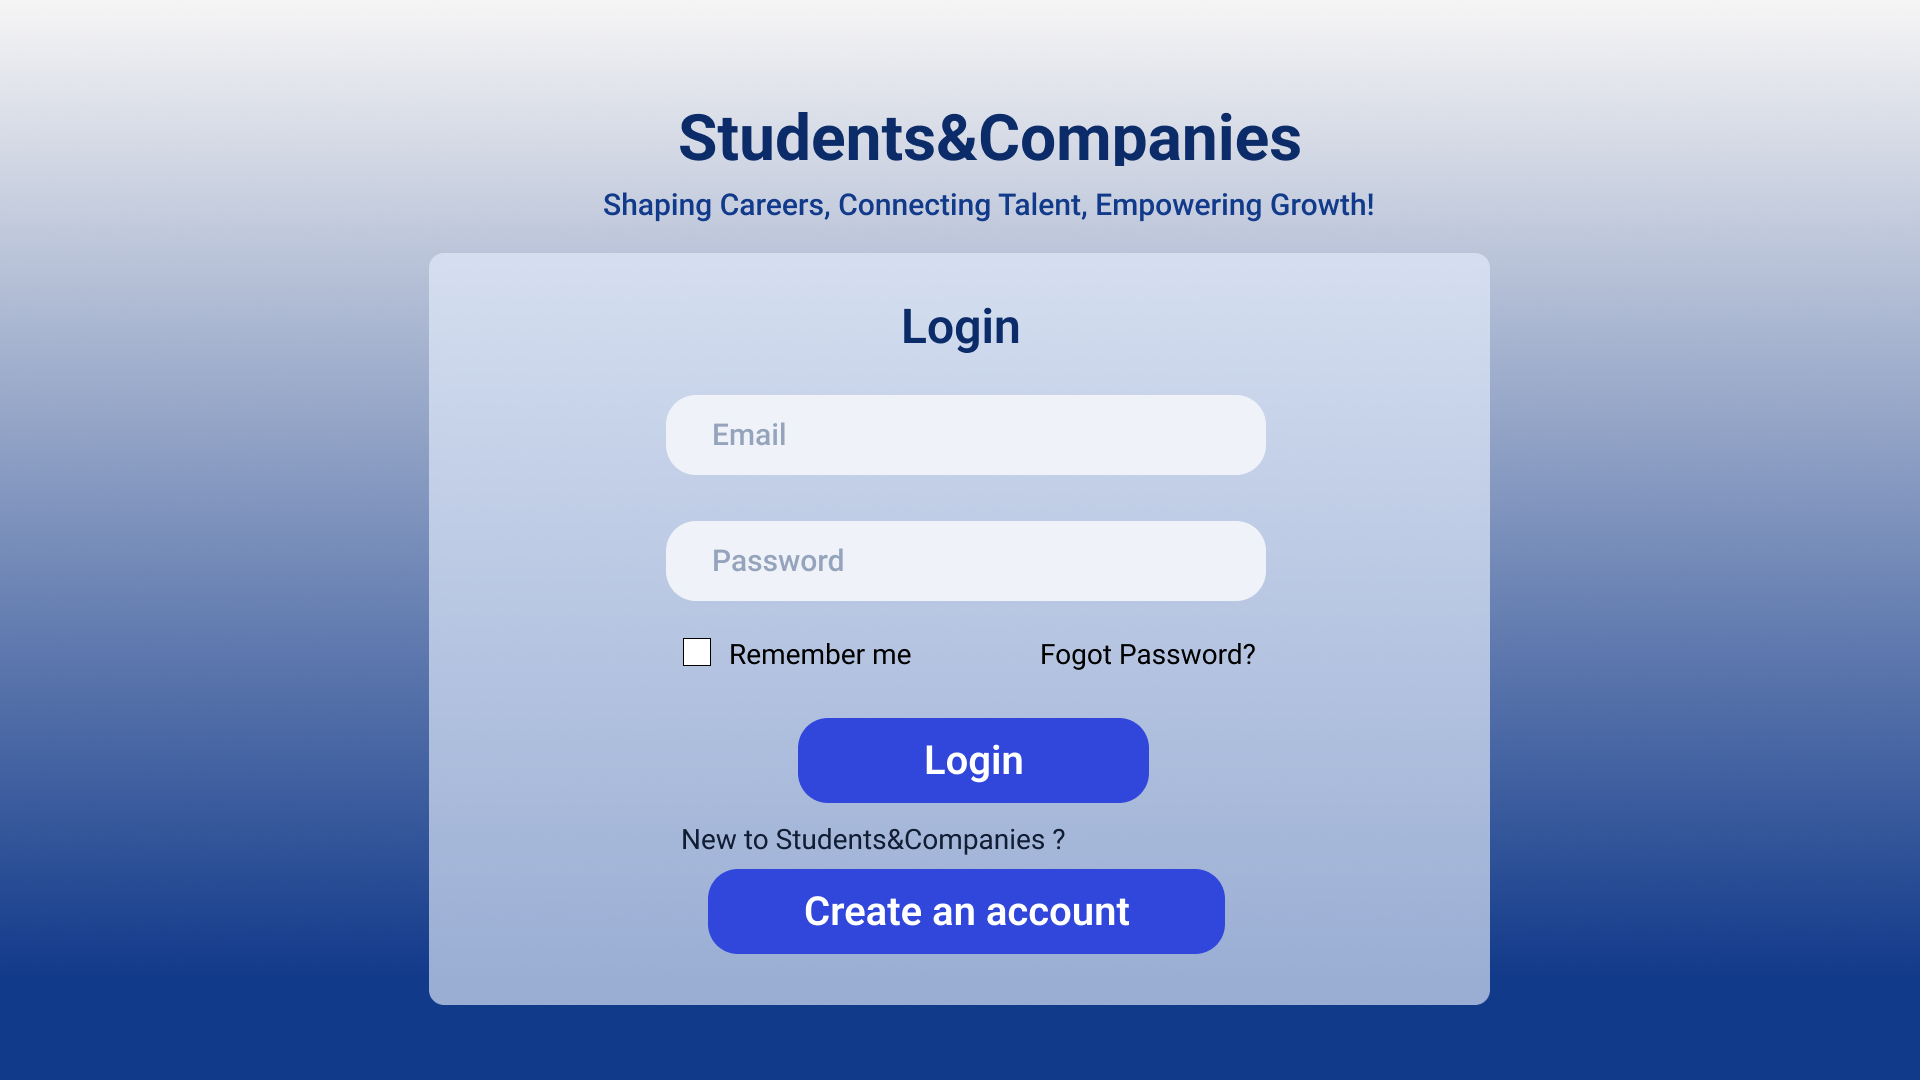
\includegraphics[width=0.8\textwidth]{Images/UI/Welcome Page.png}
    \caption{Welcome Page}\label{fig:Welcome_page}
\end{figure}

\subsection{Register Page}
If the User is not registered and wants to create an account, they will be asked to choose the type of account they want to create. 
Clicking on the type listed will redirect to the corresponding Register Page where the user can fill in the required information.
\begin{figure}[H]
    \centering
    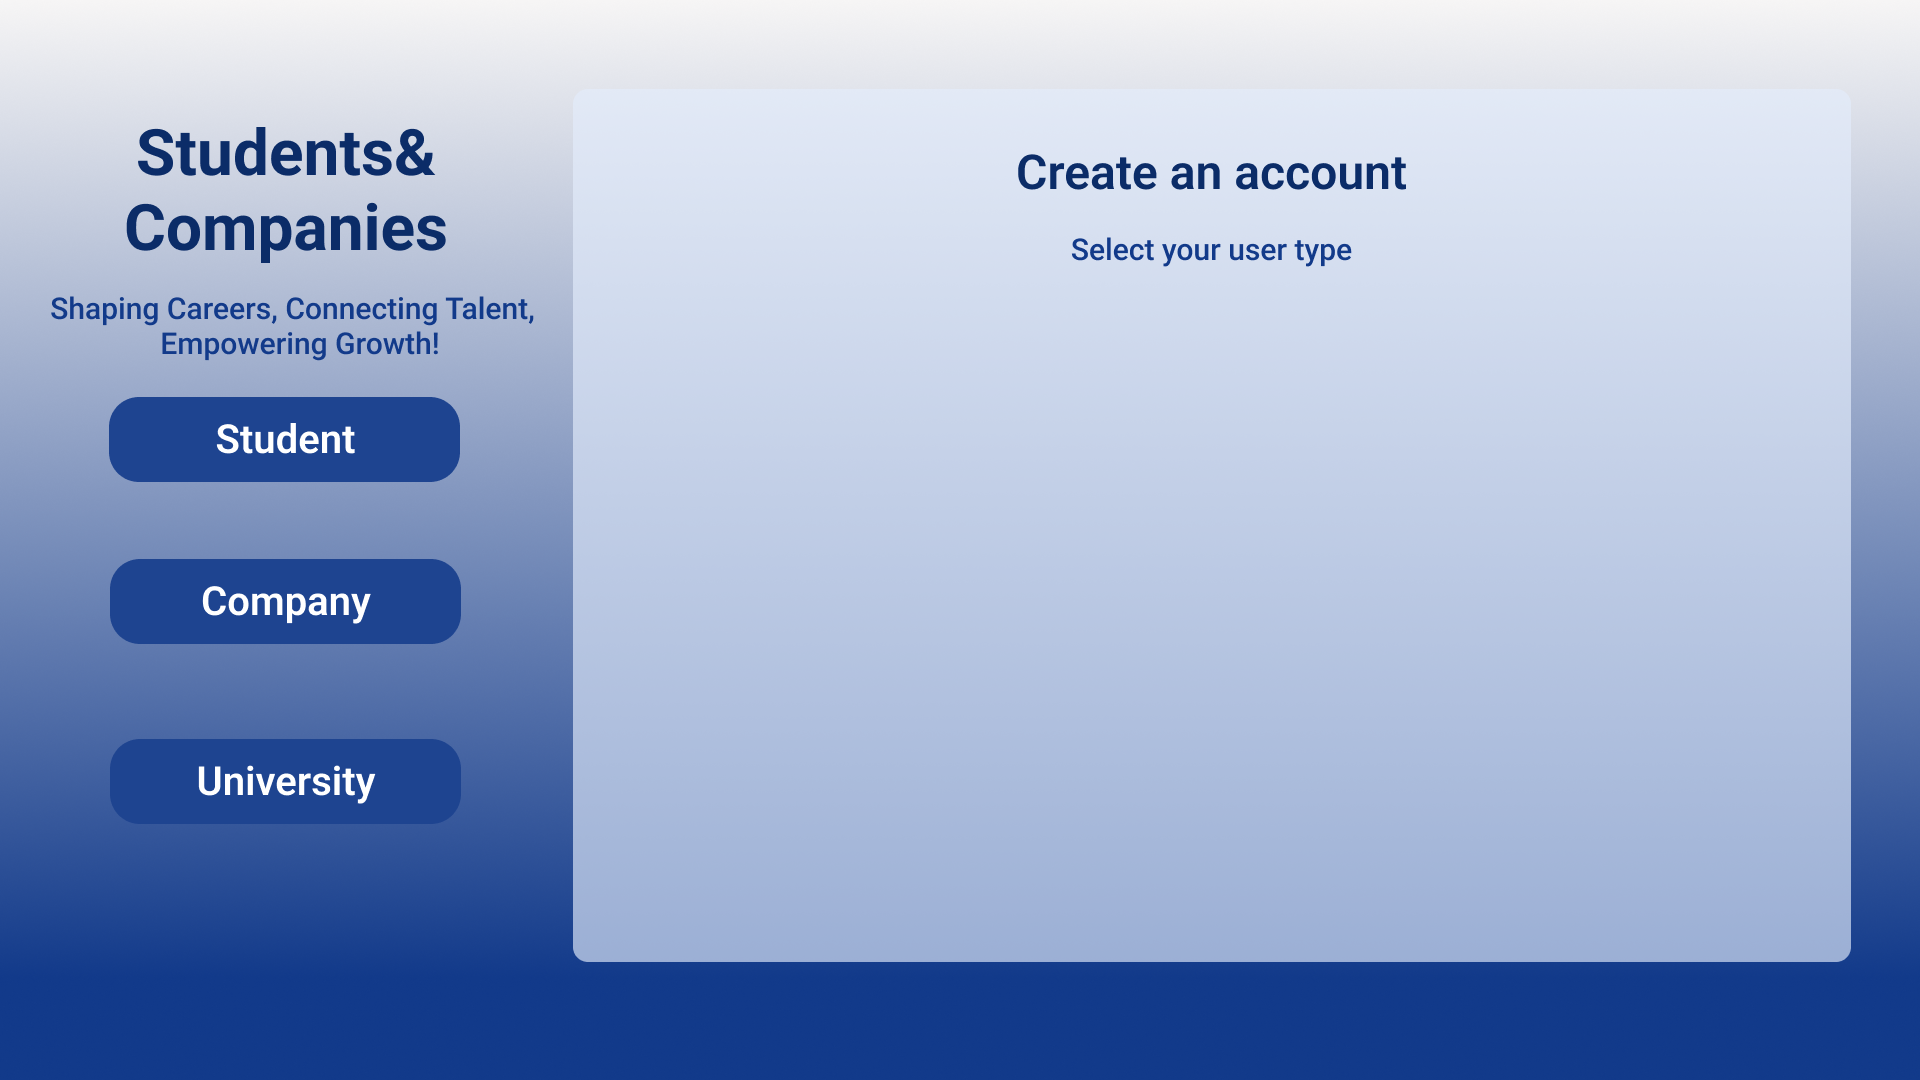
\includegraphics[width=0.8\textwidth]{Images/UI/Create account.png}
    \caption{Register Page}\label{fig:Creat_account}
\end{figure}

\begin{figure}[H]
    \centering
    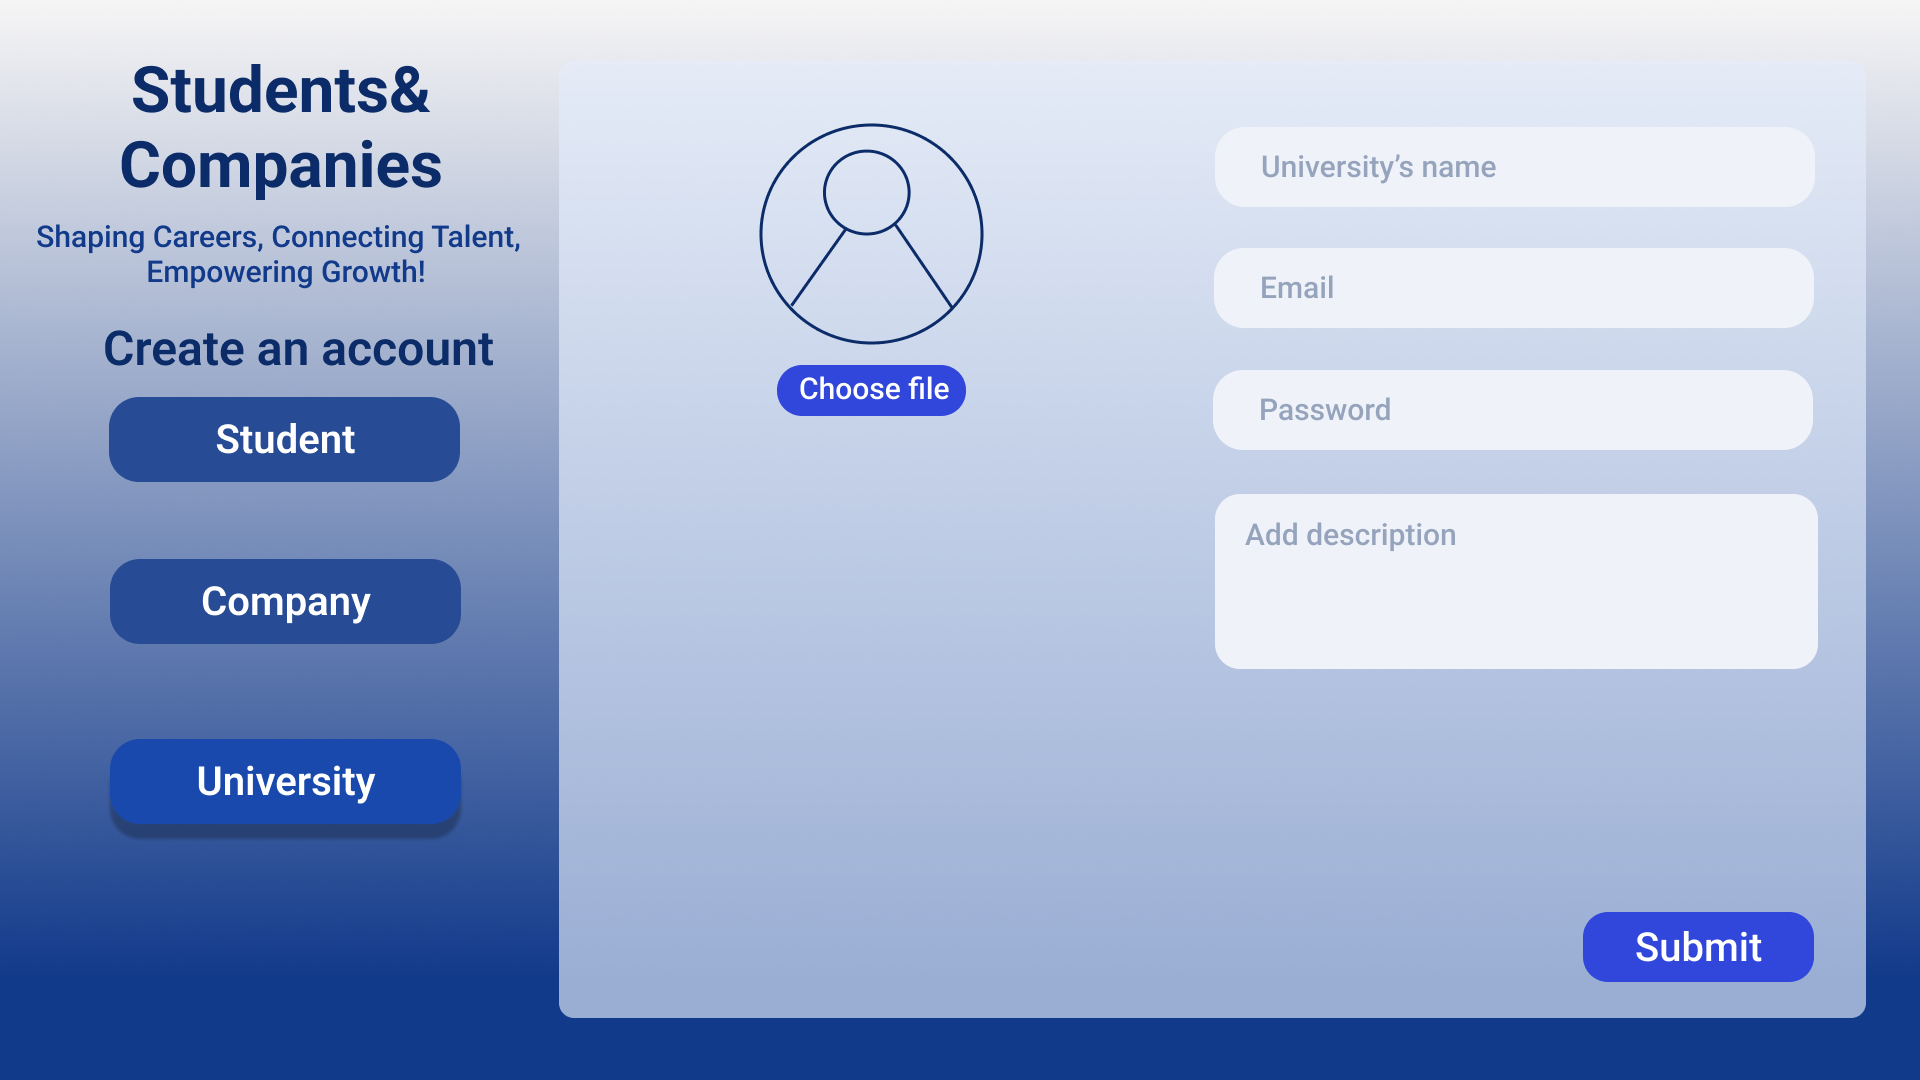
\includegraphics[width=0.8\textwidth]{Images/UI/Create account University.png}
    \caption{University create account}\label{fig:Creat_account University}
\end{figure}

\begin{figure}[H]
    \centering
    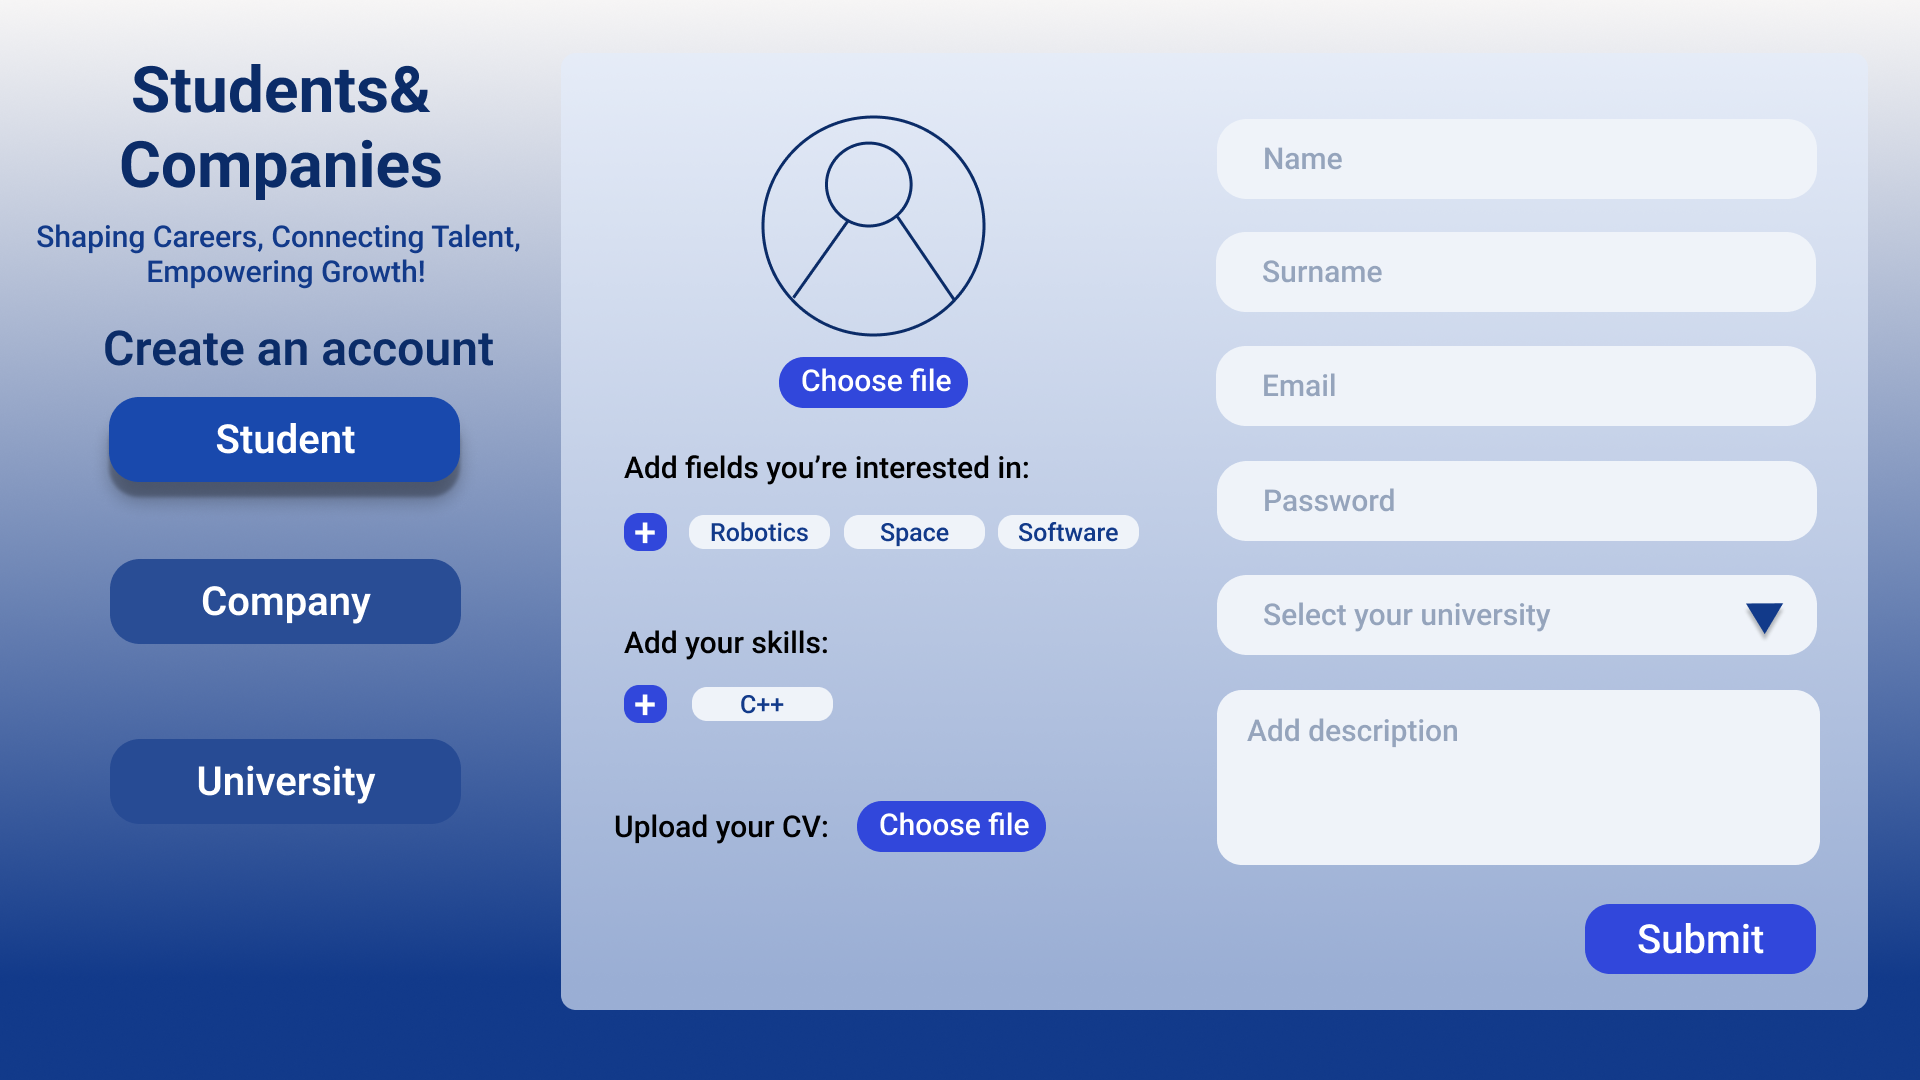
\includegraphics[width=0.8\textwidth]{Images/UI/Create account student.png}
    \caption{Student create account}\label{fig:Creat_account student}
\end{figure}

\begin{figure}[H]
    \centering
    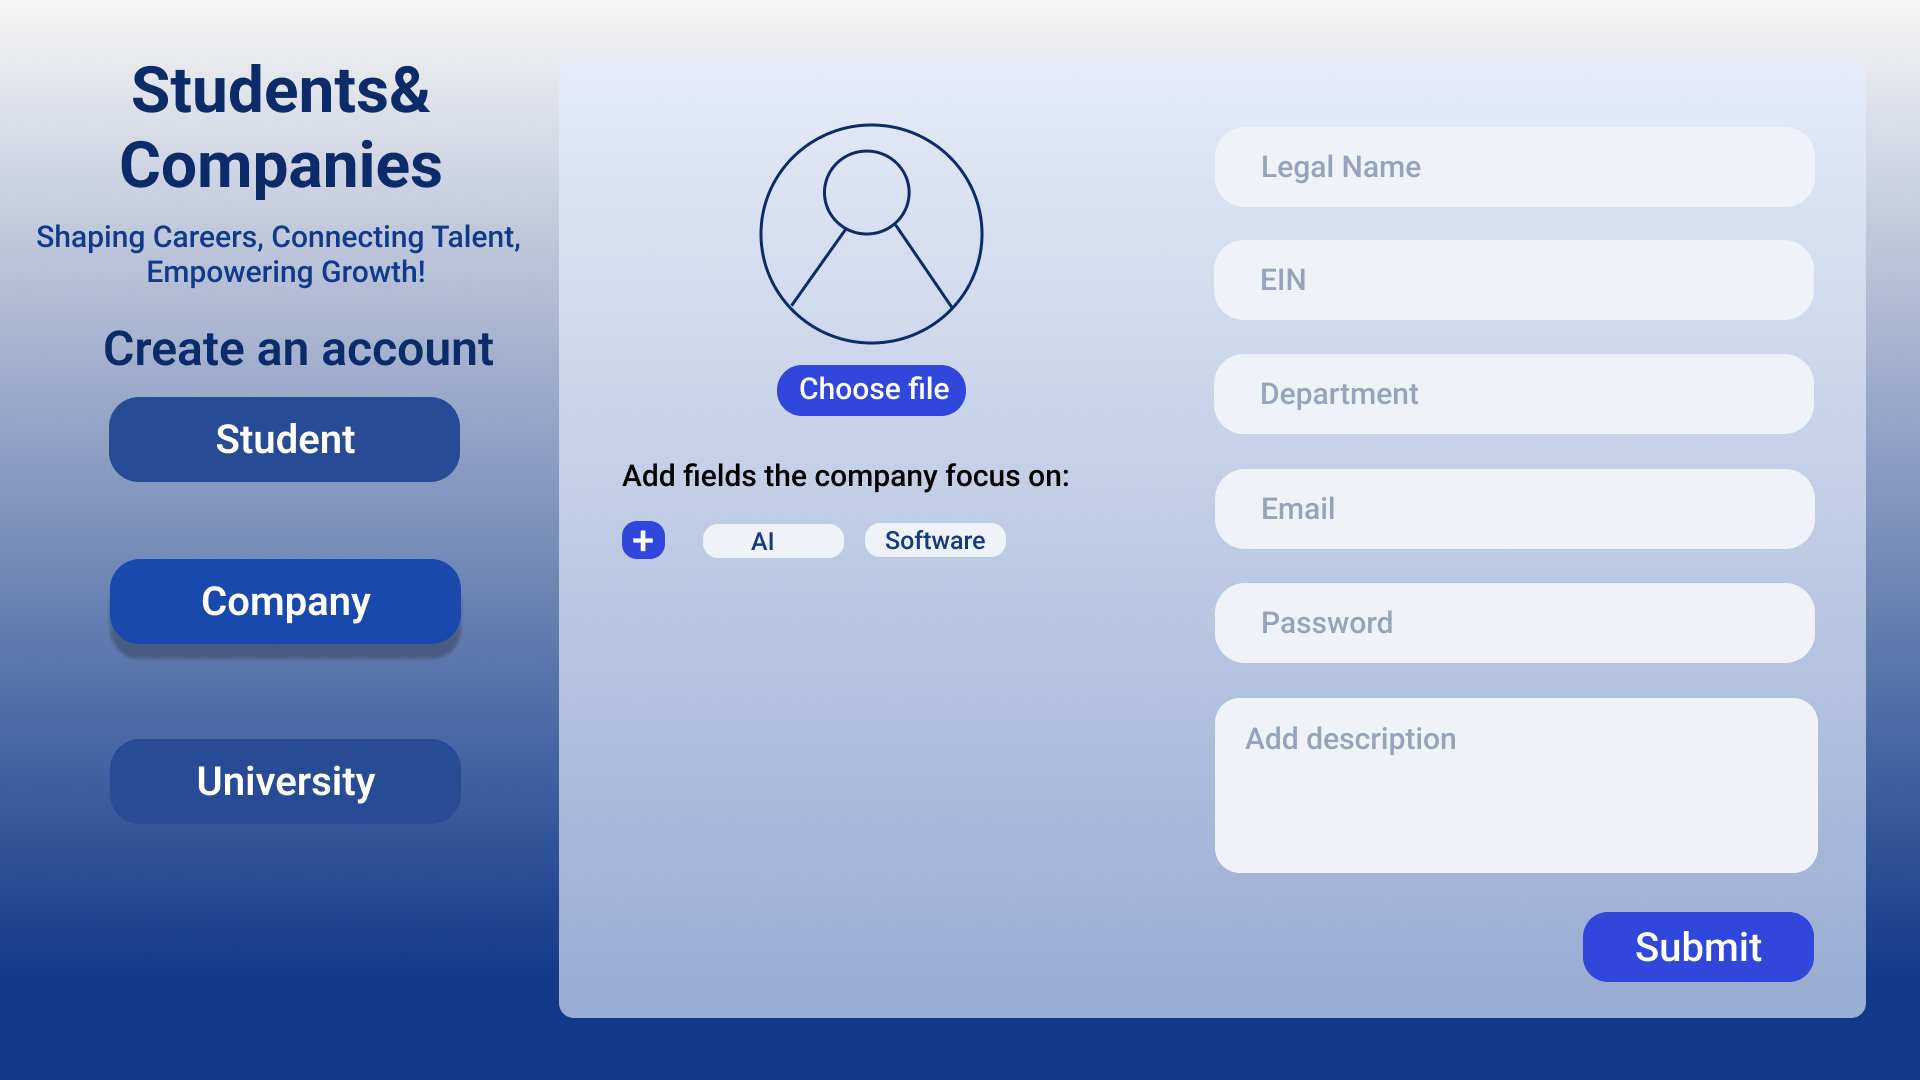
\includegraphics[width=0.8\textwidth]{Images/UI/Create account company.png}
    \caption{Company create account}\label{fig:Creat_account company}
\end{figure}

\subsection{Student's view}
Once access to the platform, to optimizing the user experience, the student will be able to use the side menu to navigate the main 
functionalities provided by the platform to satisfy their needs. 
\begin{figure}[H]
    \centering
    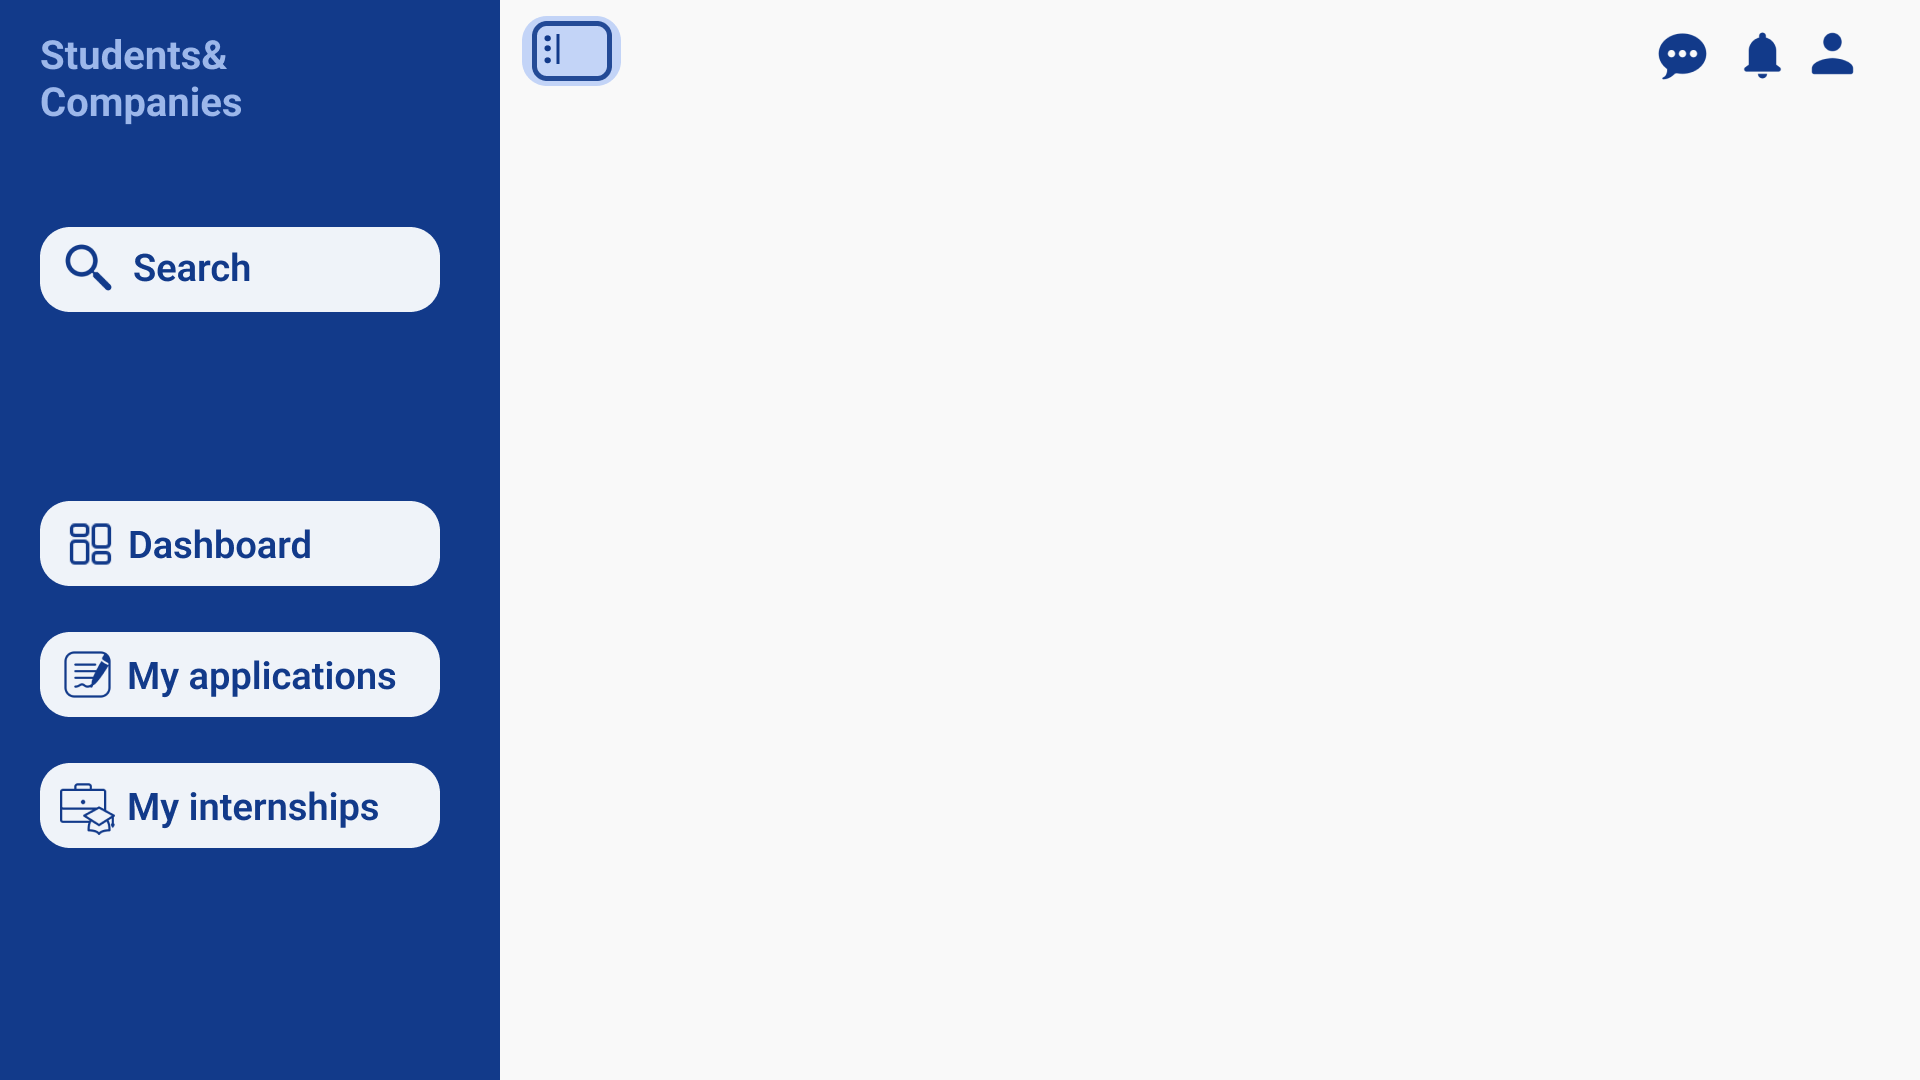
\includegraphics[width=0.8\textwidth]{Images/UI/Layout-Student.png}
    \caption{Student's Side Menu}\label{fig:Student_view}
\end{figure}
By default, the student will be directed to the Dashboard page once logged in. %%To be continued
\begin{figure}[H]
    \centering
    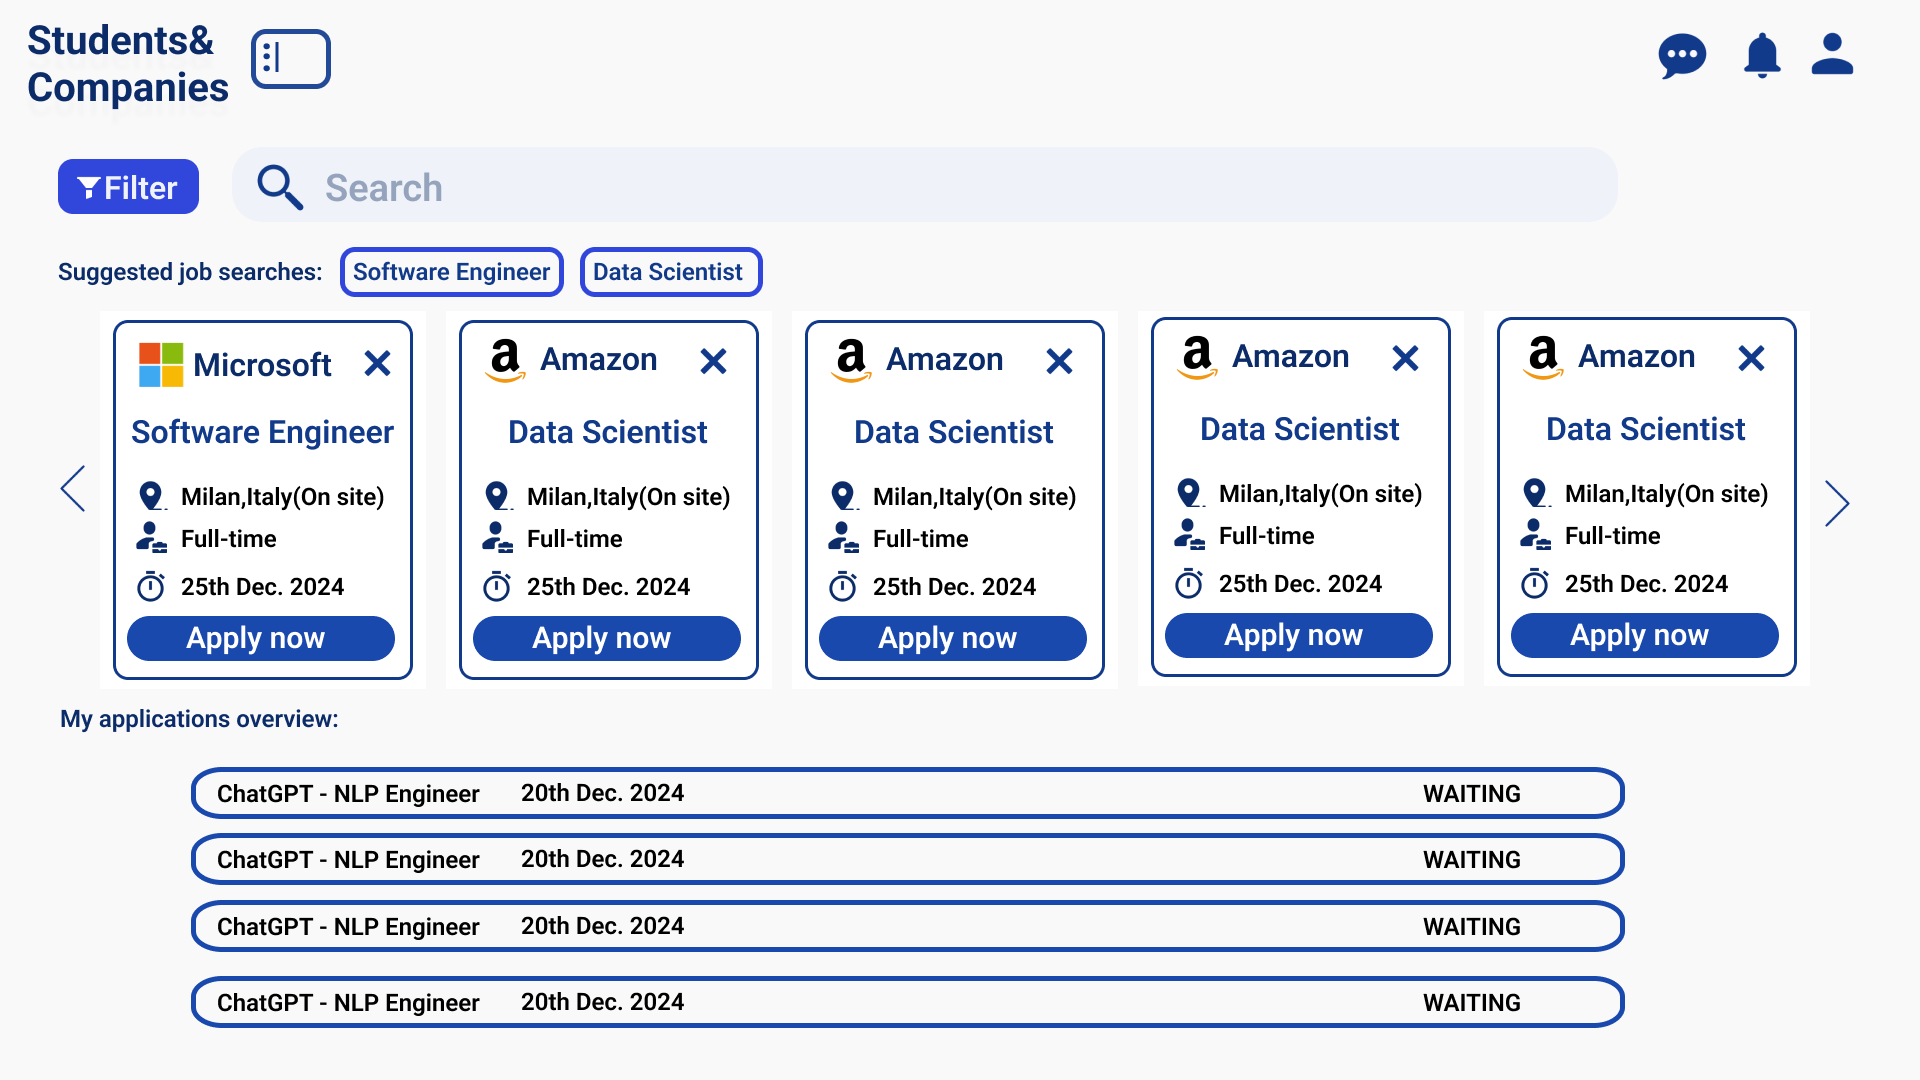
\includegraphics[width=0.8\textwidth]{Images/UI/Dashboard 1-student.png}
    \caption{Student's Dashboard 1}\label{fig:DashboardStudent1}
\end{figure}

\begin{figure}[H]
    \centering
    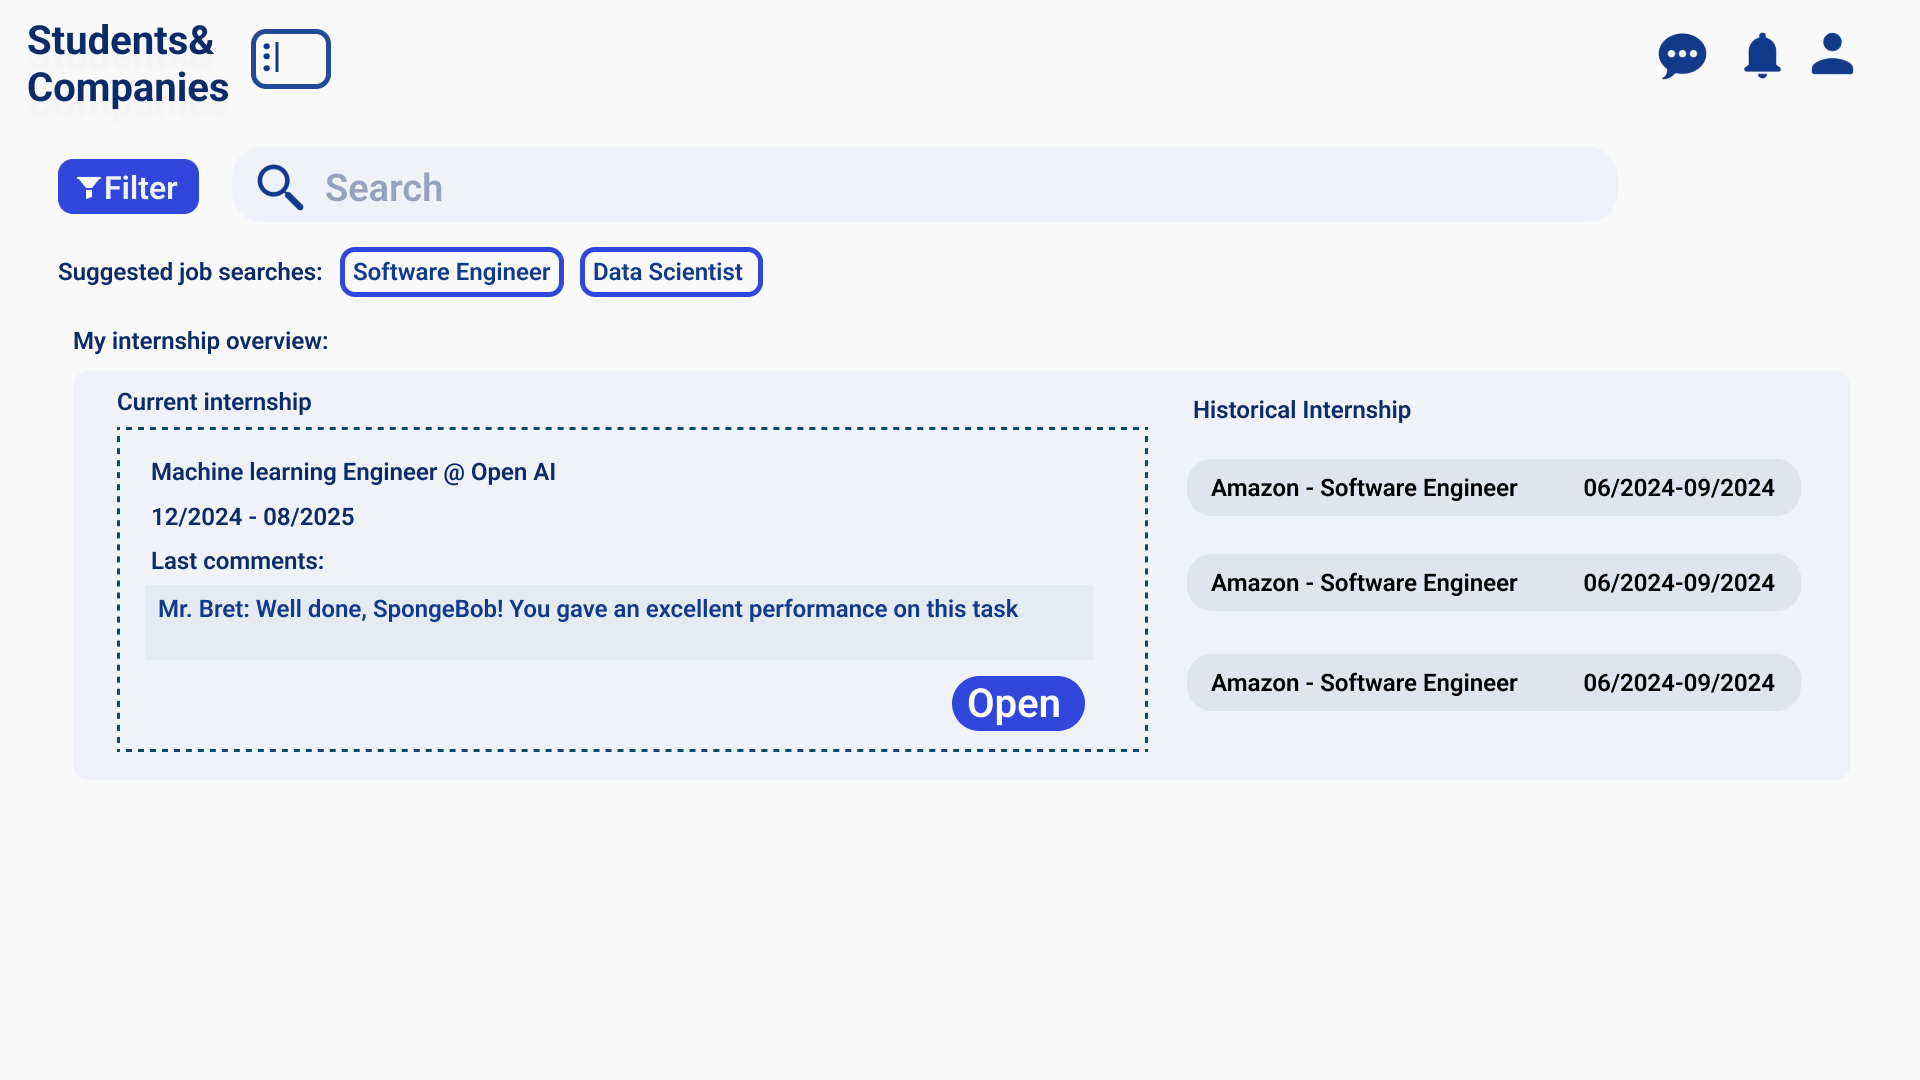
\includegraphics[width=0.8\textwidth]{Images/UI/Dashboard 2-student.png}
    \caption{Student's Dashboard 2}\label{fig:Dashboard Student 2}
\end{figure}

\begin{figure}[H]
    \centering
    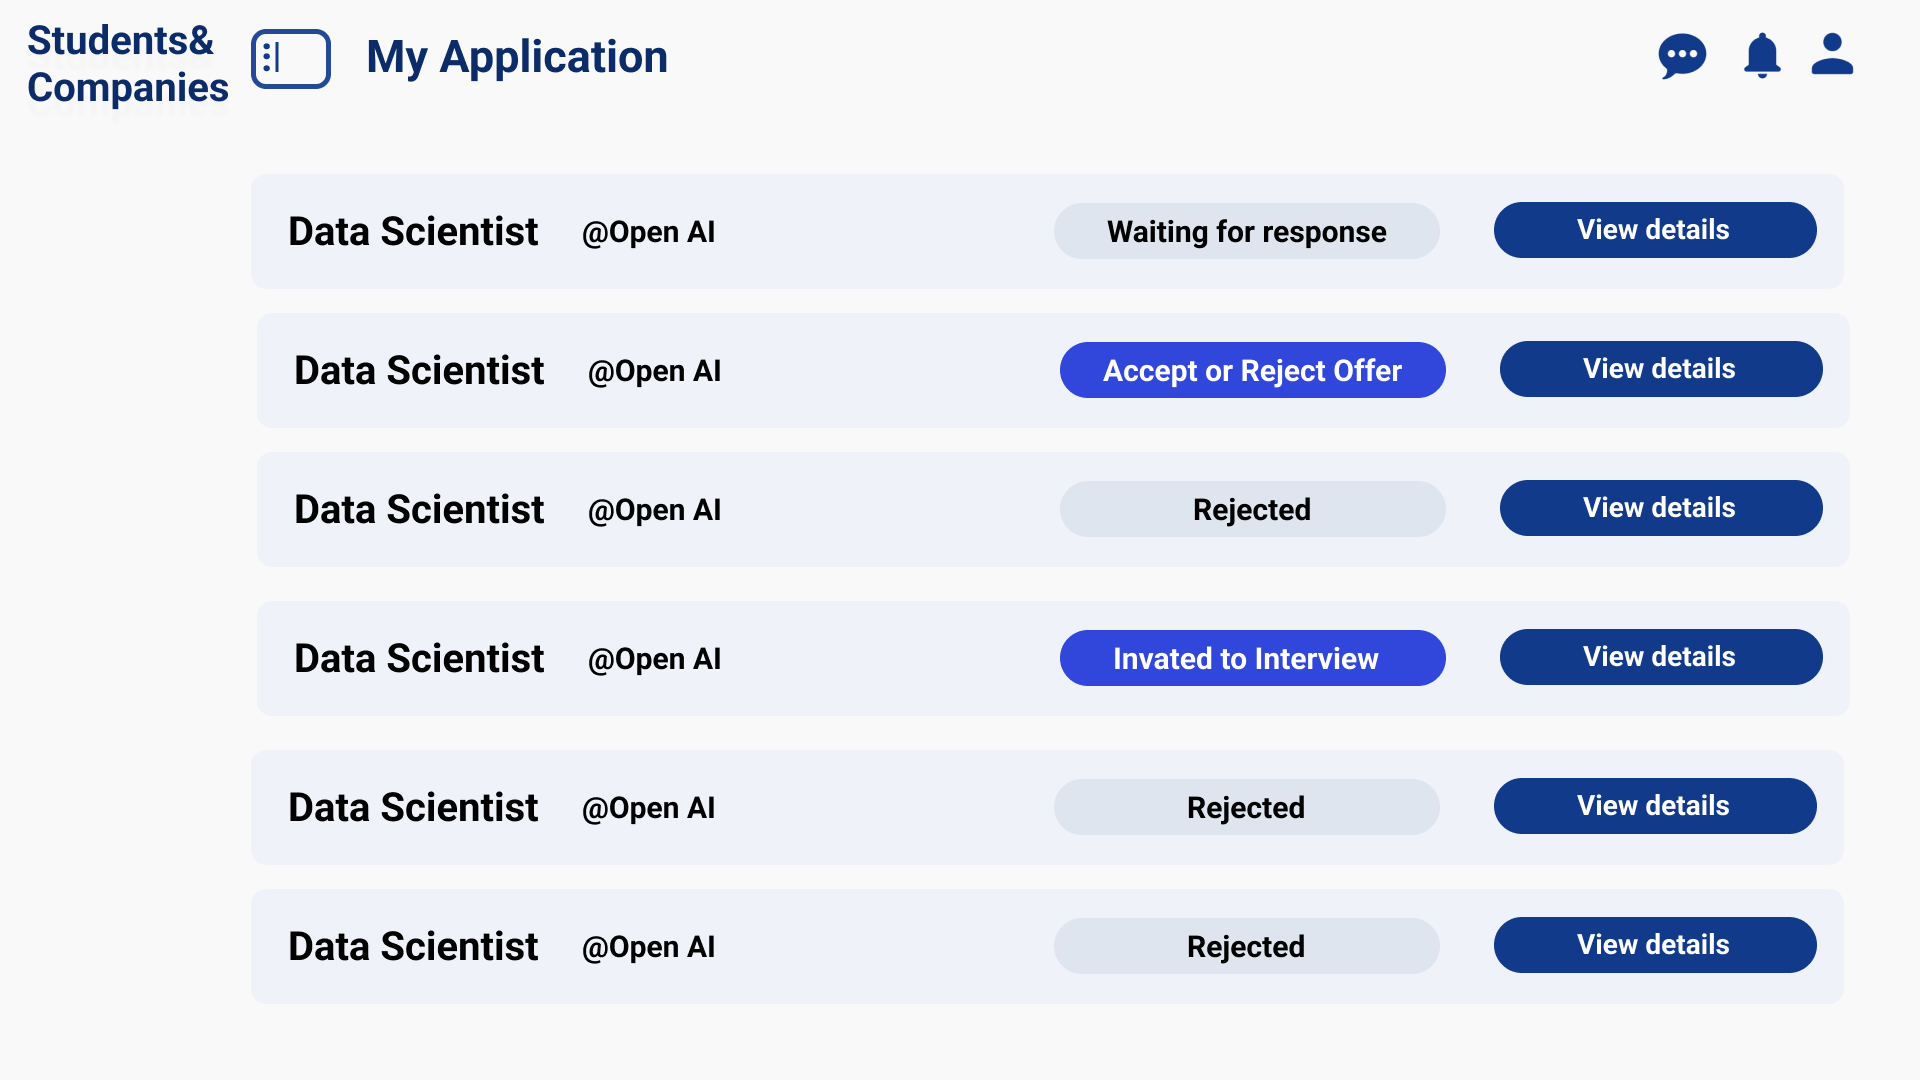
\includegraphics[width=0.8\textwidth]{Images/UI/My Application-student.png}
    \caption{My application}\label{fig:My application}
\end{figure}

\begin{figure}[H]
    \centering
    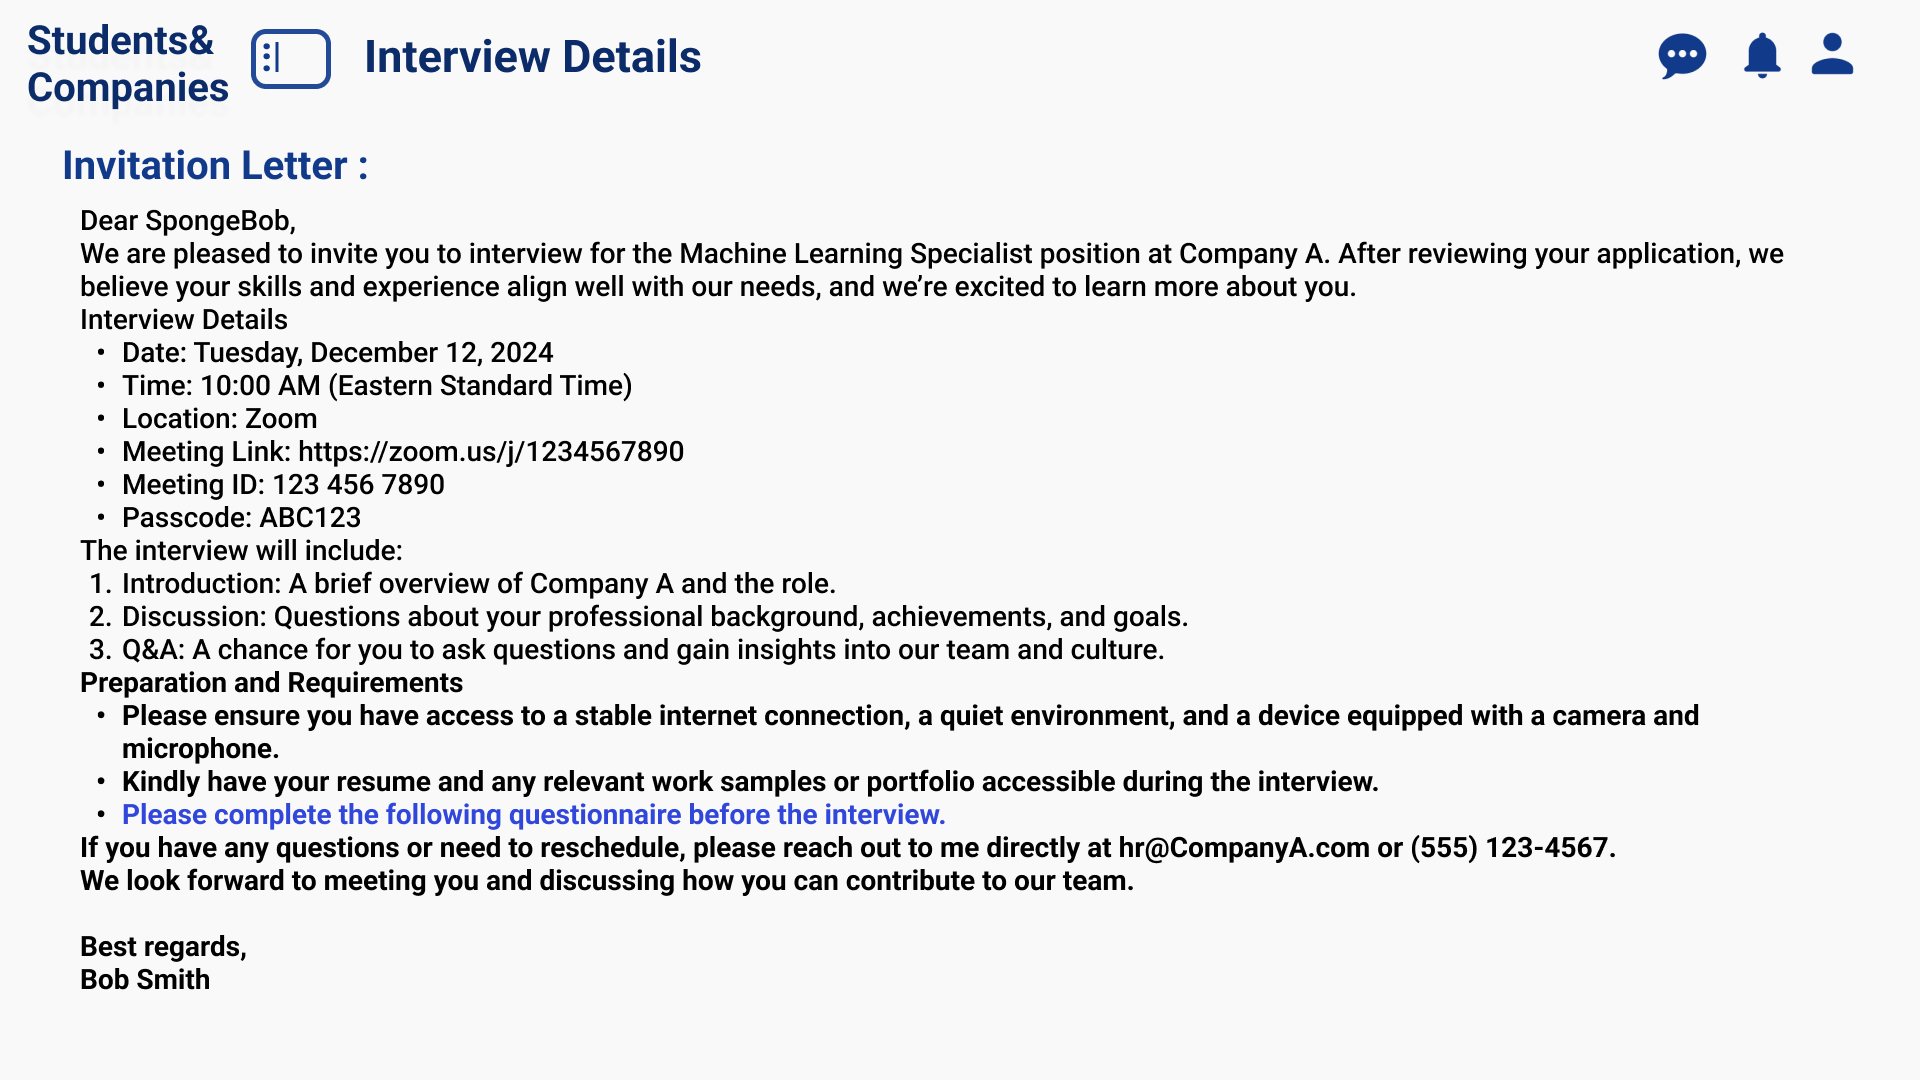
\includegraphics[width=0.8\textwidth]{Images/UI/Interview Details-student.png}
    \caption{Interview details 1}\label{fig:Interview details 1}
\end{figure}

\begin{figure}[H]
    \centering
    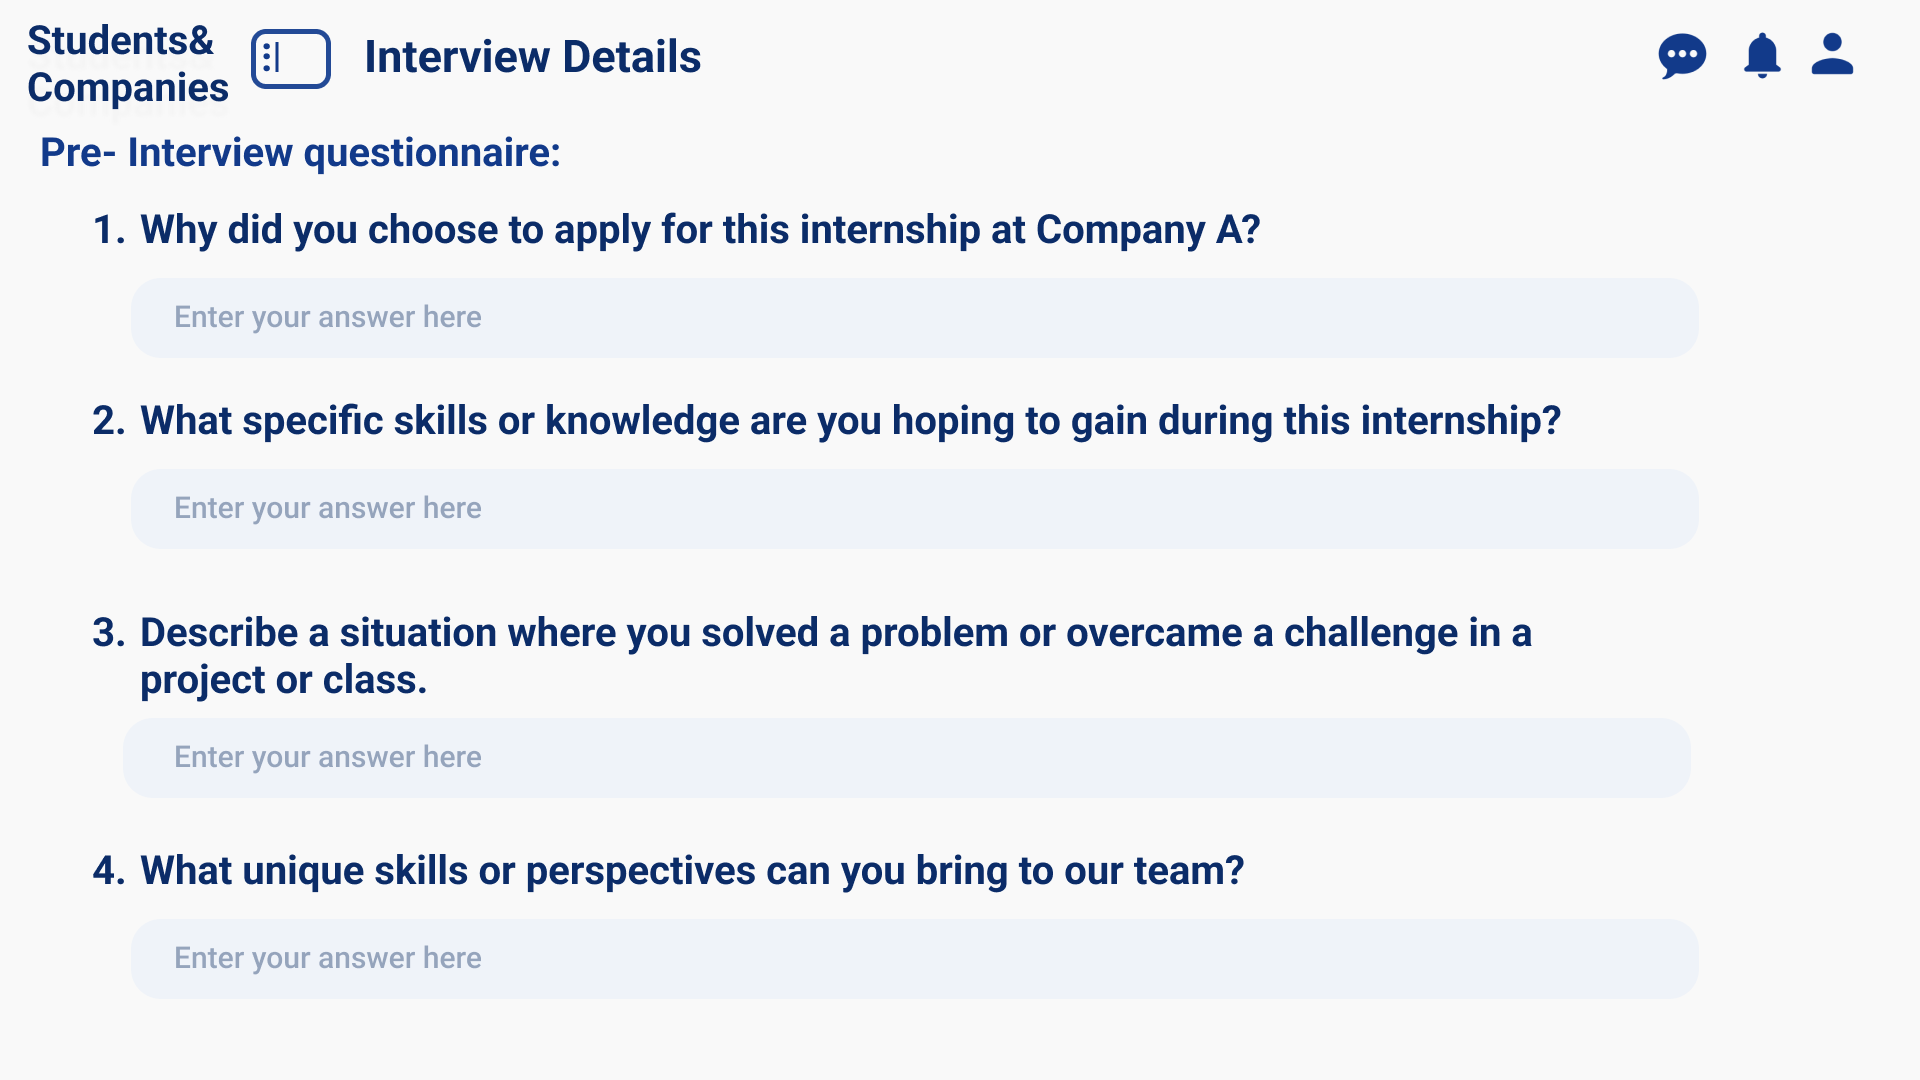
\includegraphics[width=0.8\textwidth]{Images/UI/Interview Details2-student.png}
    \caption{Interview details 2}\label{fig:Interview details 2}
\end{figure}

\begin{figure}[H]
    \centering
    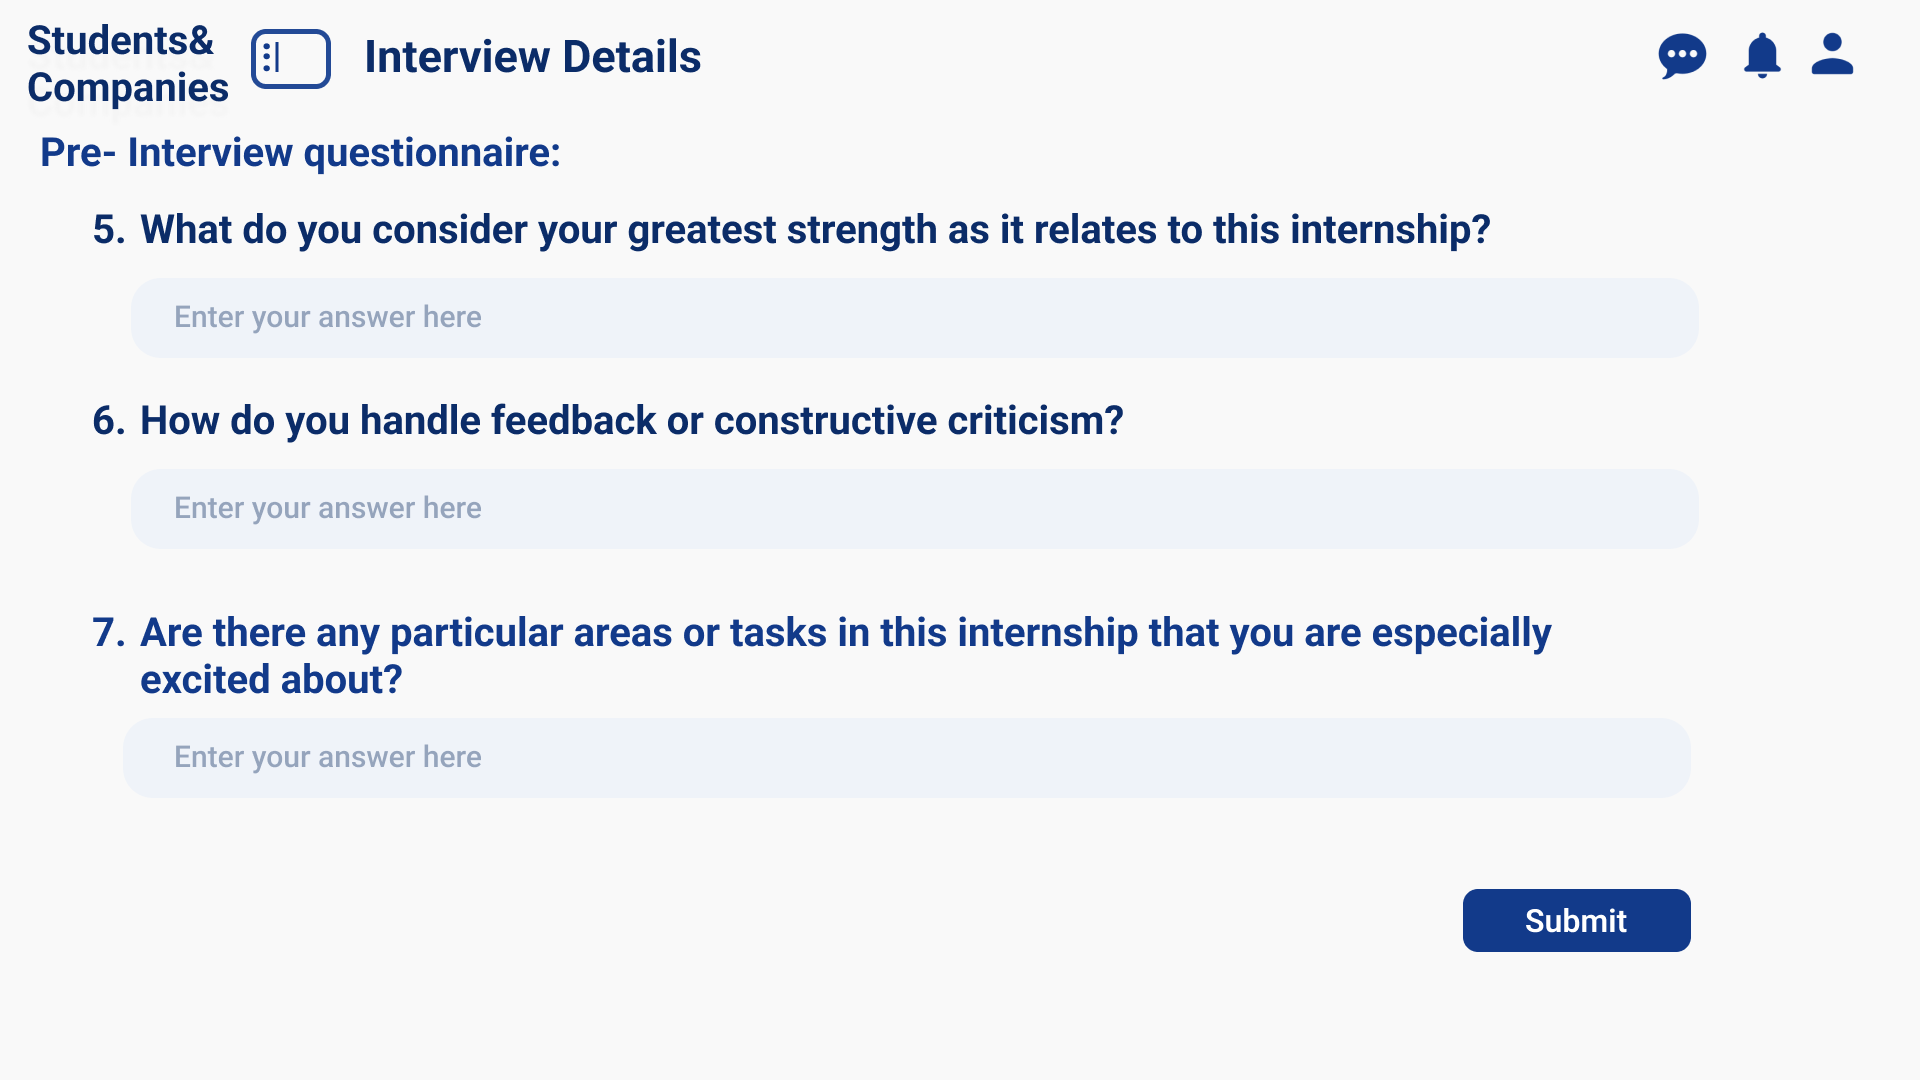
\includegraphics[width=0.8\textwidth]{Images/UI/Interview Details3-student.png}
    \caption{Interview details 3}\label{fig:Interview details 3}
\end{figure}

\begin{figure}[H]
    \centering
    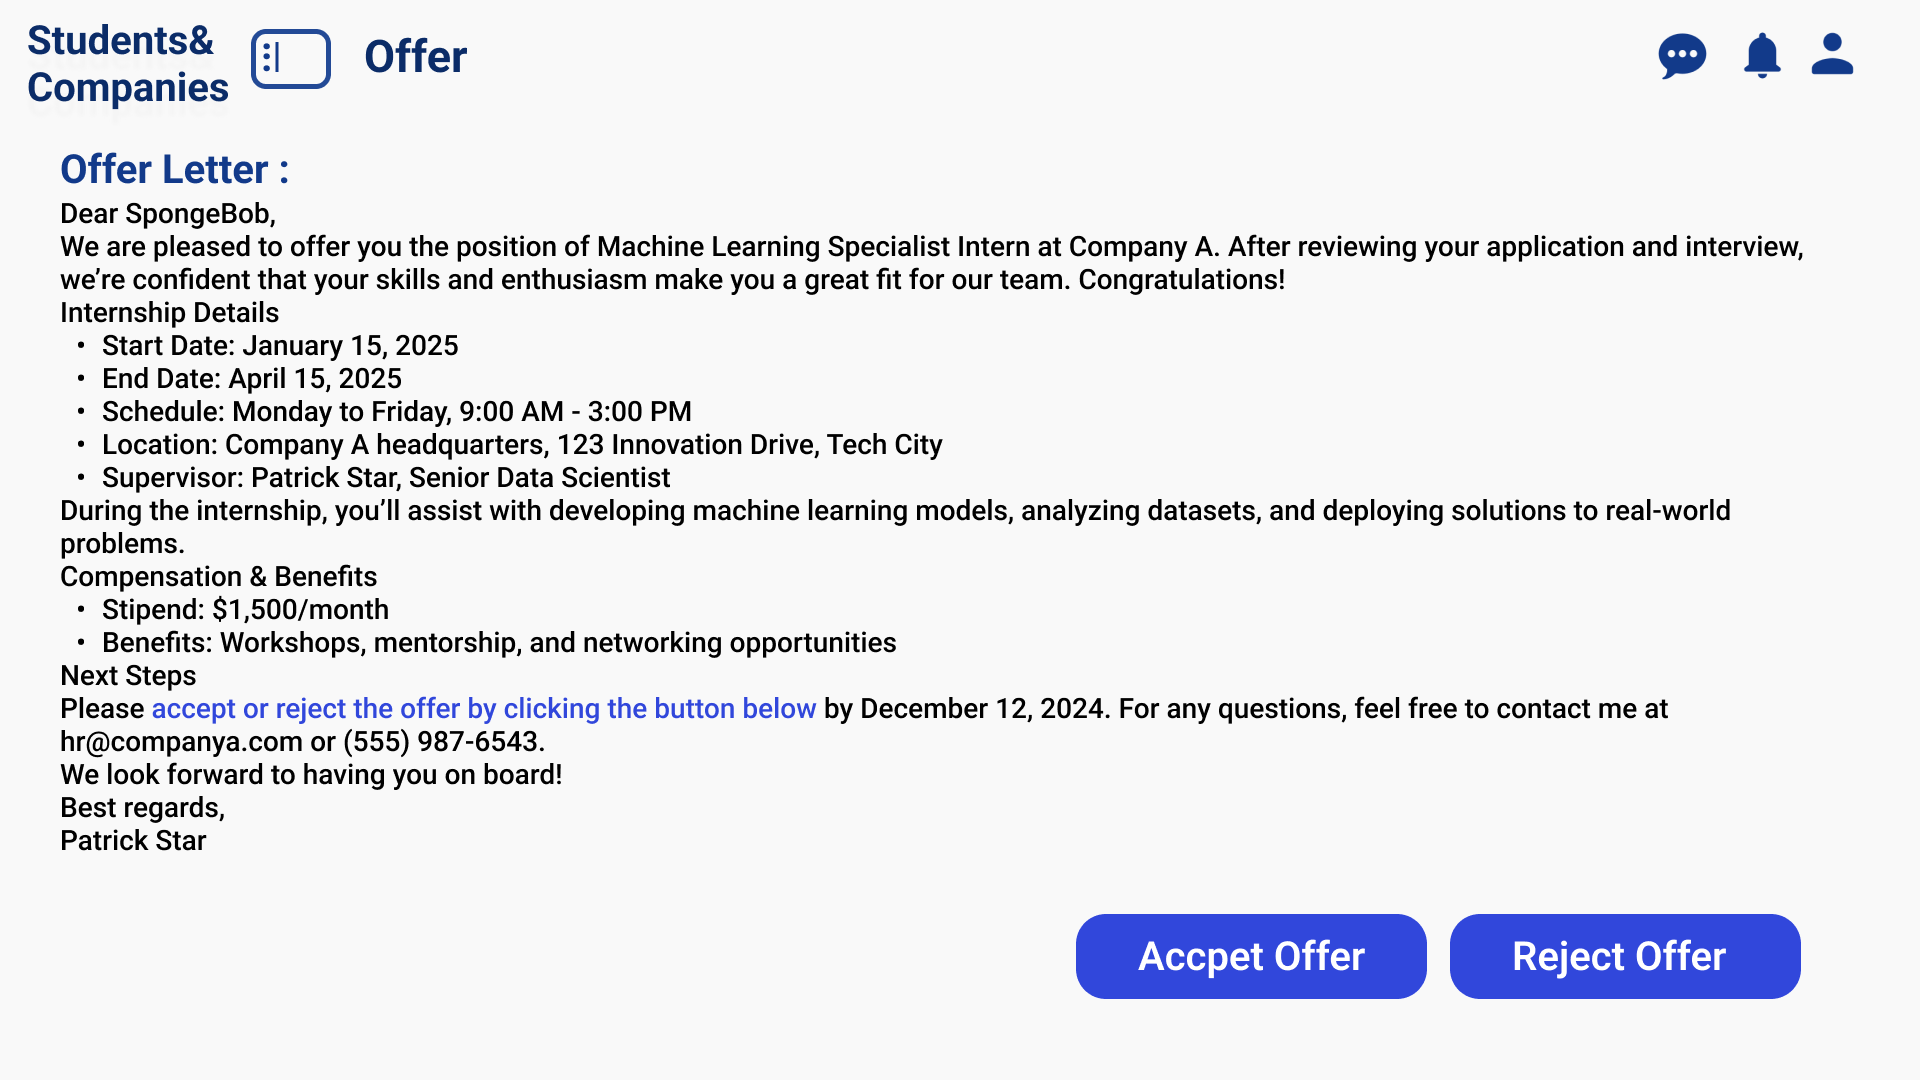
\includegraphics[width=0.8\textwidth]{Images/UI/Reject-student.png}
    \caption{Accept or Reject Offer }\label{fig:Accept or Reject Offer}
\end{figure}

\begin{figure}[H]
    \centering
    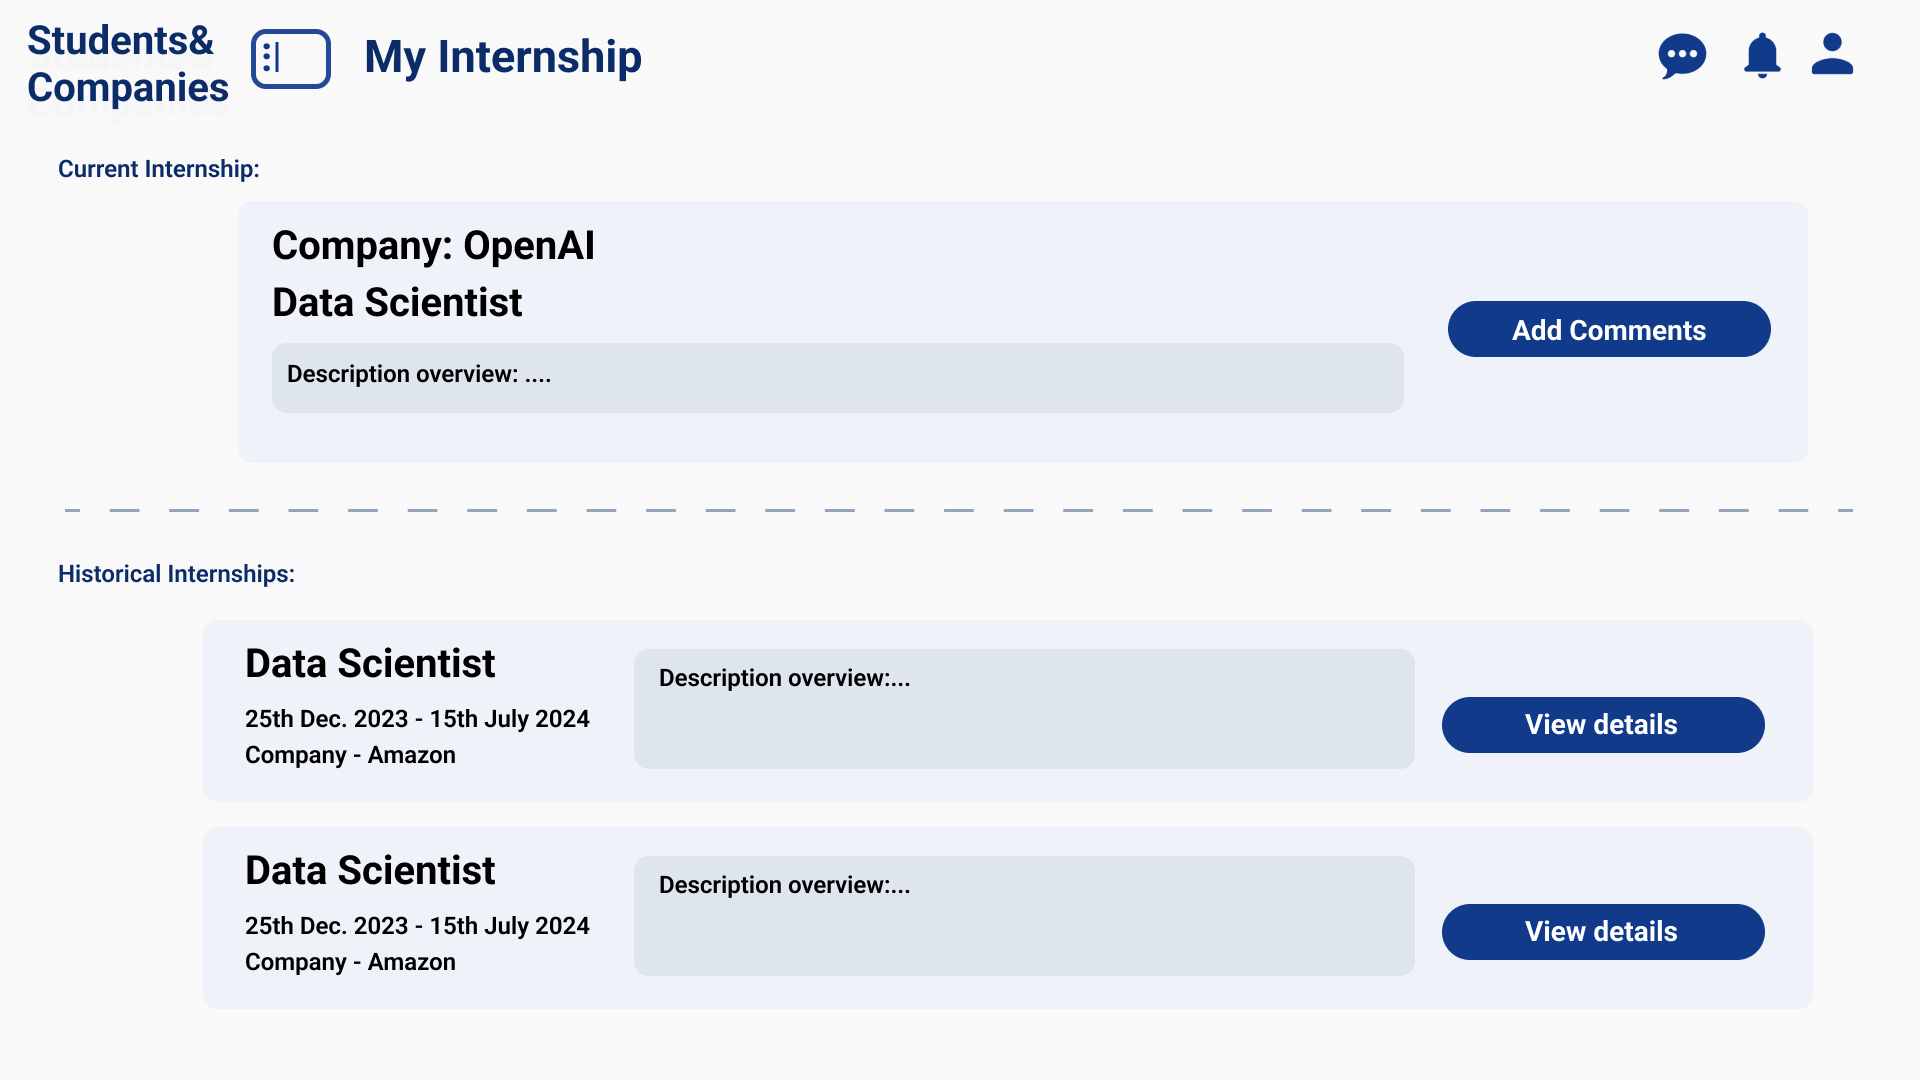
\includegraphics[width=0.8\textwidth]{Images/UI/My Internship-student.png}
    \caption{My internship }\label{fig:My internship}
\end{figure}

\begin{figure}[H]
    \centering
    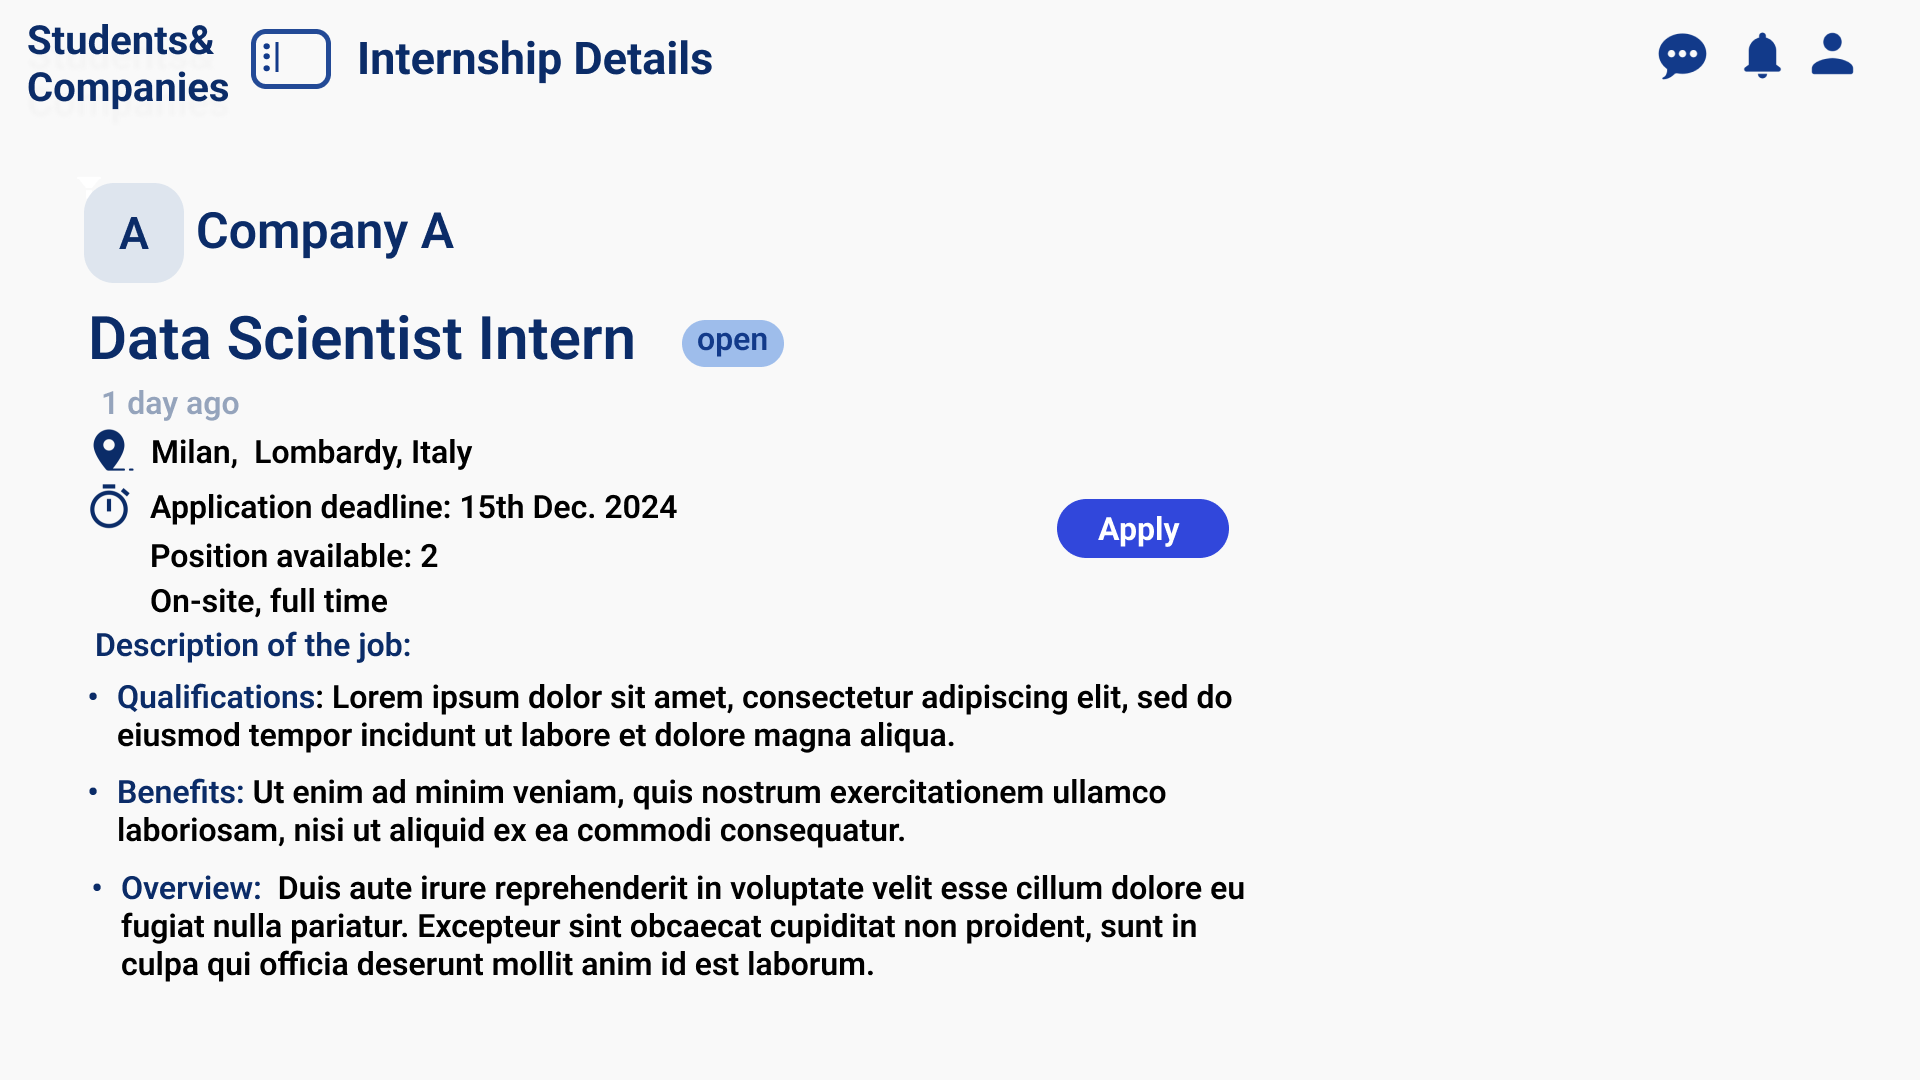
\includegraphics[width=0.8\textwidth]{Images/UI/Internship details-student view.png}
    \caption{Internship announcement details }\label{fig:Internship announcement details}
\end{figure}

\begin{figure}[H]
    \centering
    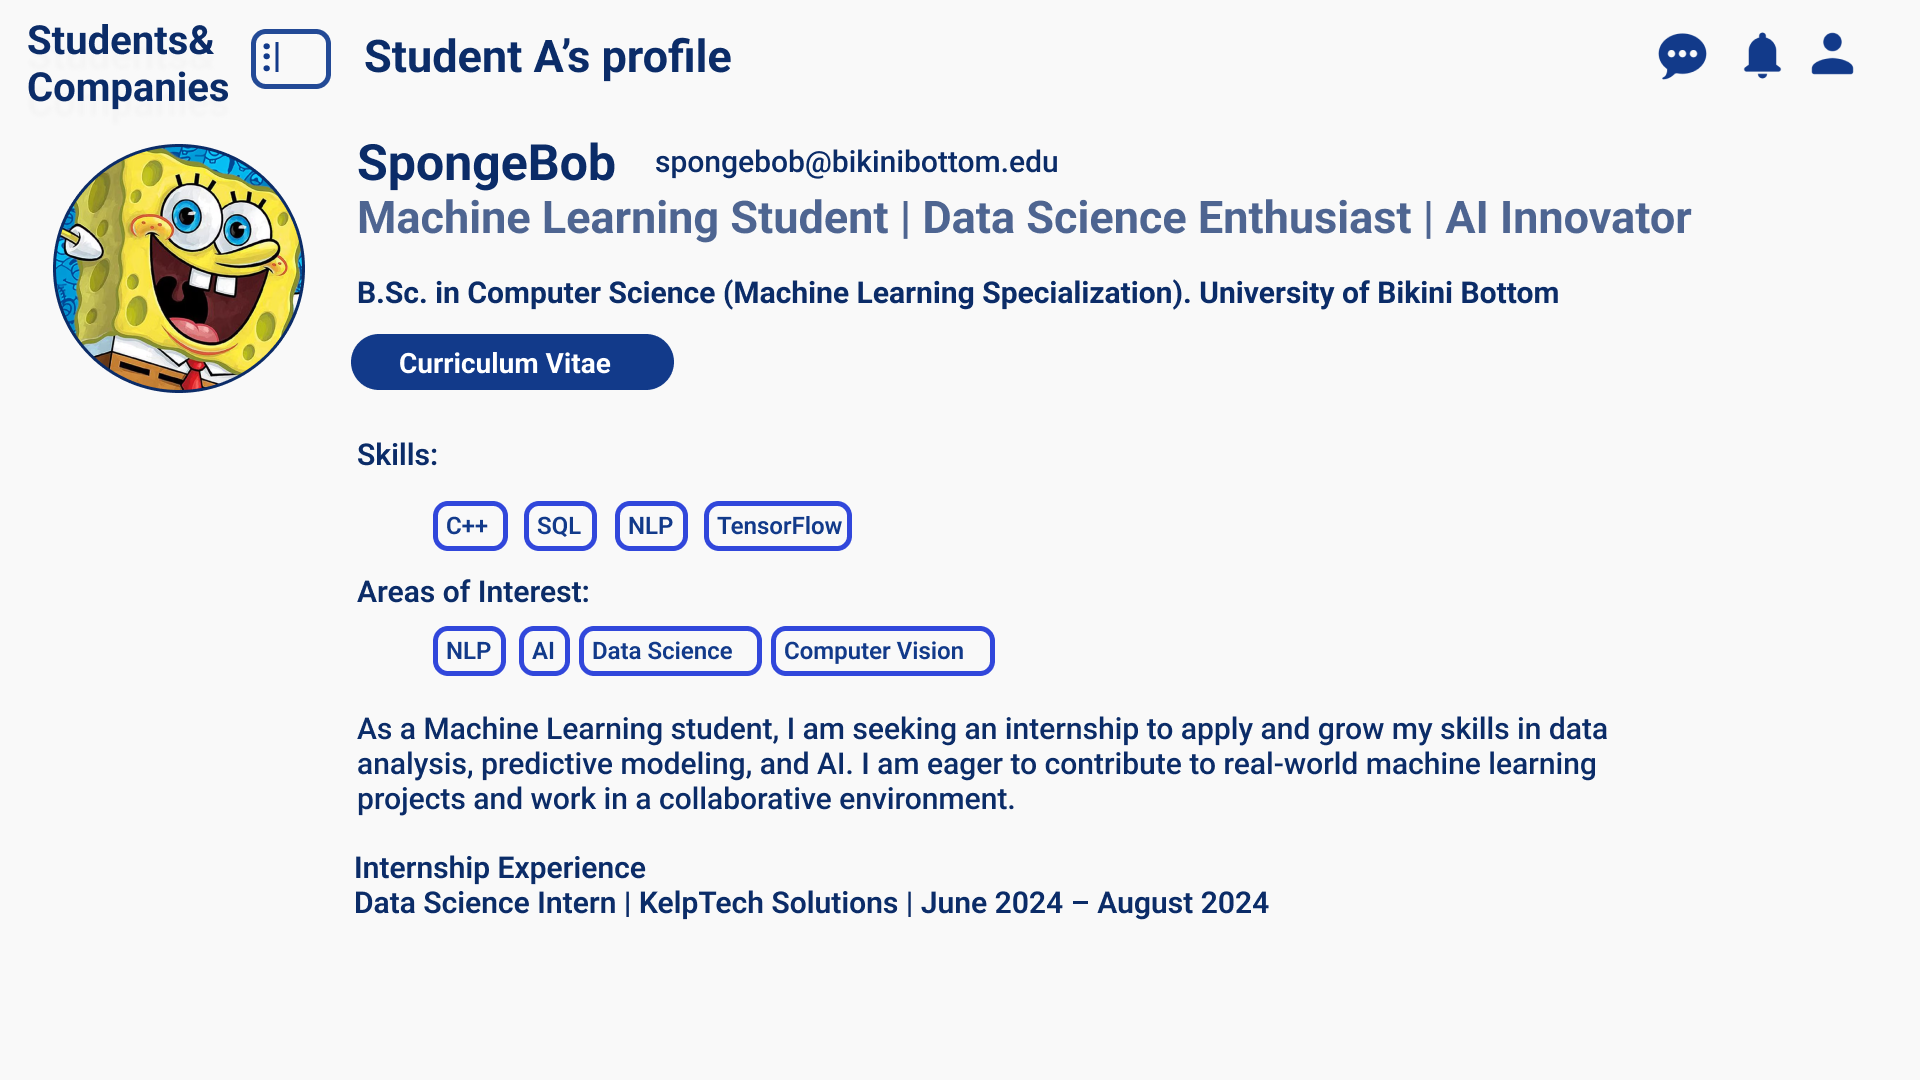
\includegraphics[width=0.8\textwidth]{Images/UI/Student profile.png}
    \caption{Student's profile from other's view}\label{fig:Student's profile from other's view}
\end{figure}

\subsection{Company's view}

\begin{figure}[H]
    \centering
    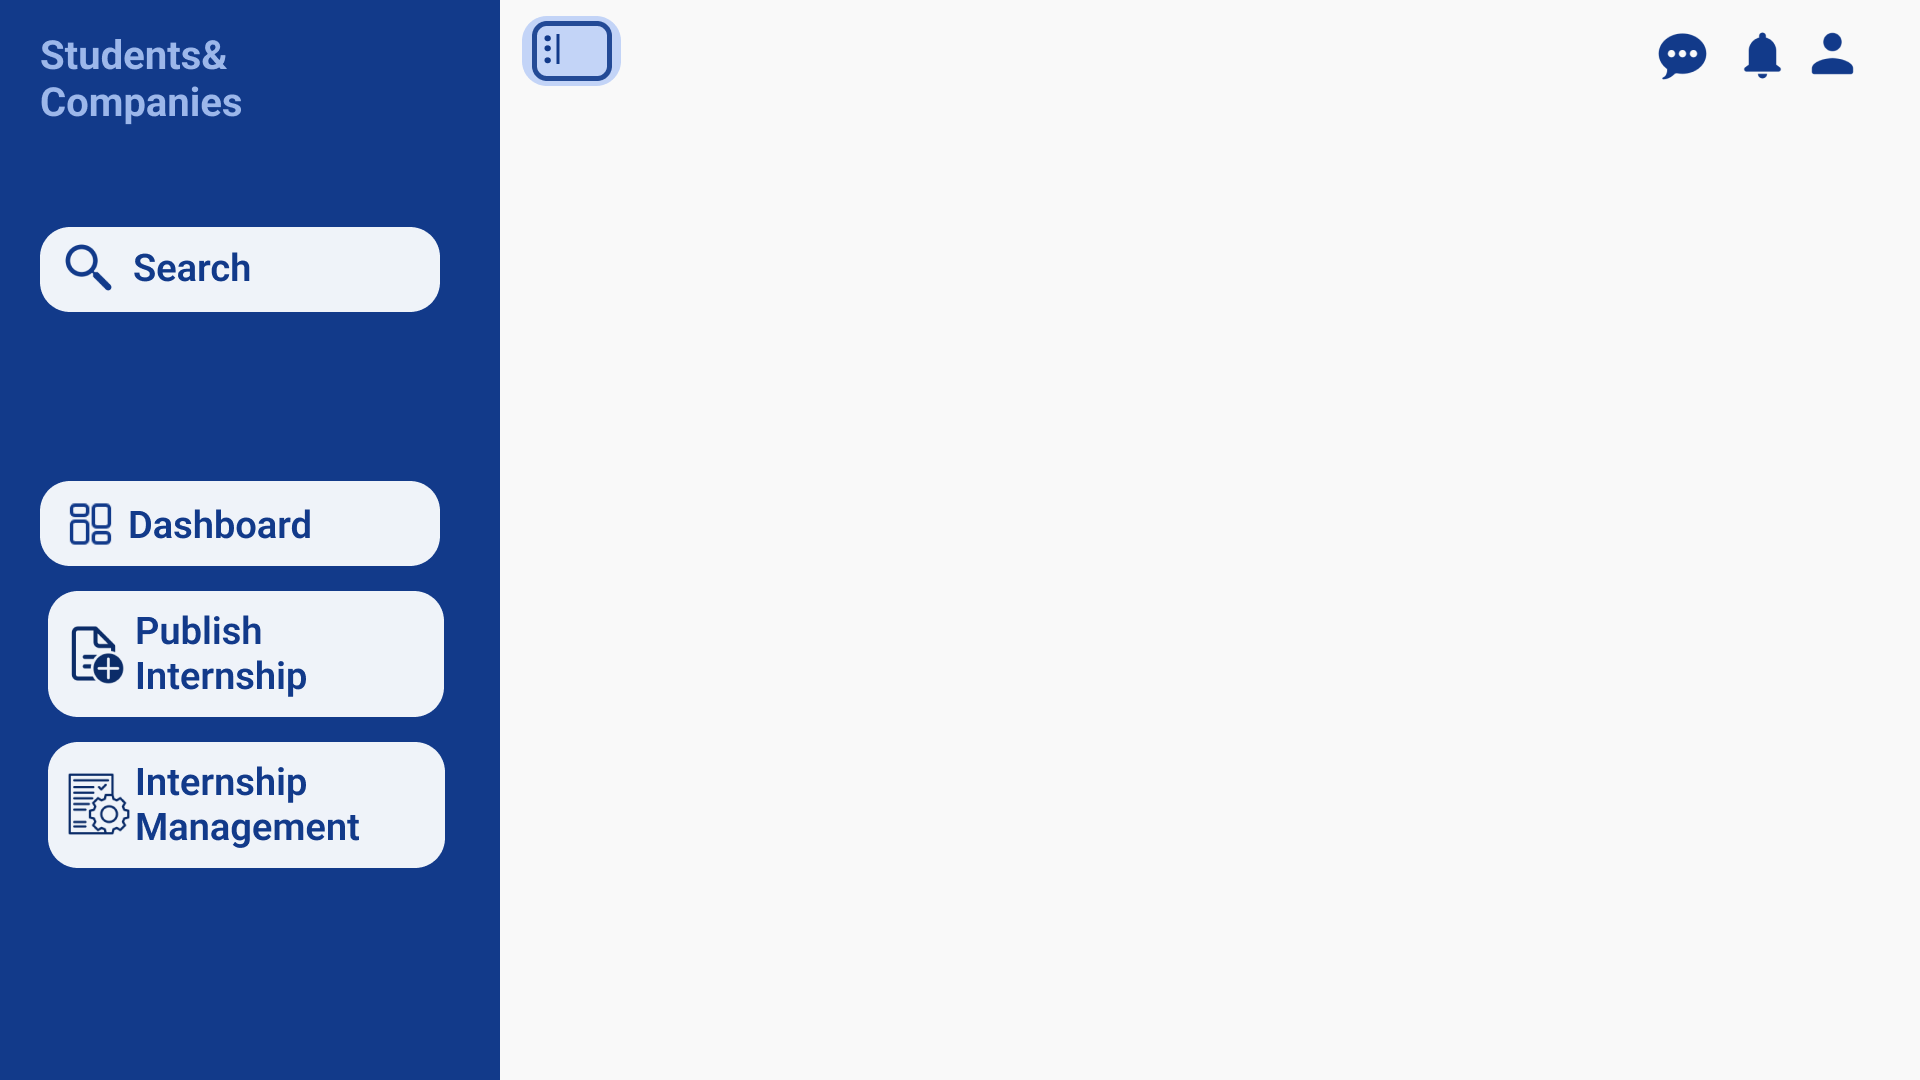
\includegraphics[width=0.8\textwidth]{Images/UI/Layout-Company.png}
    \caption{Company's Side Menu}\label{fig:Company_view}
\end{figure}

\begin{figure}[H]
    \centering
    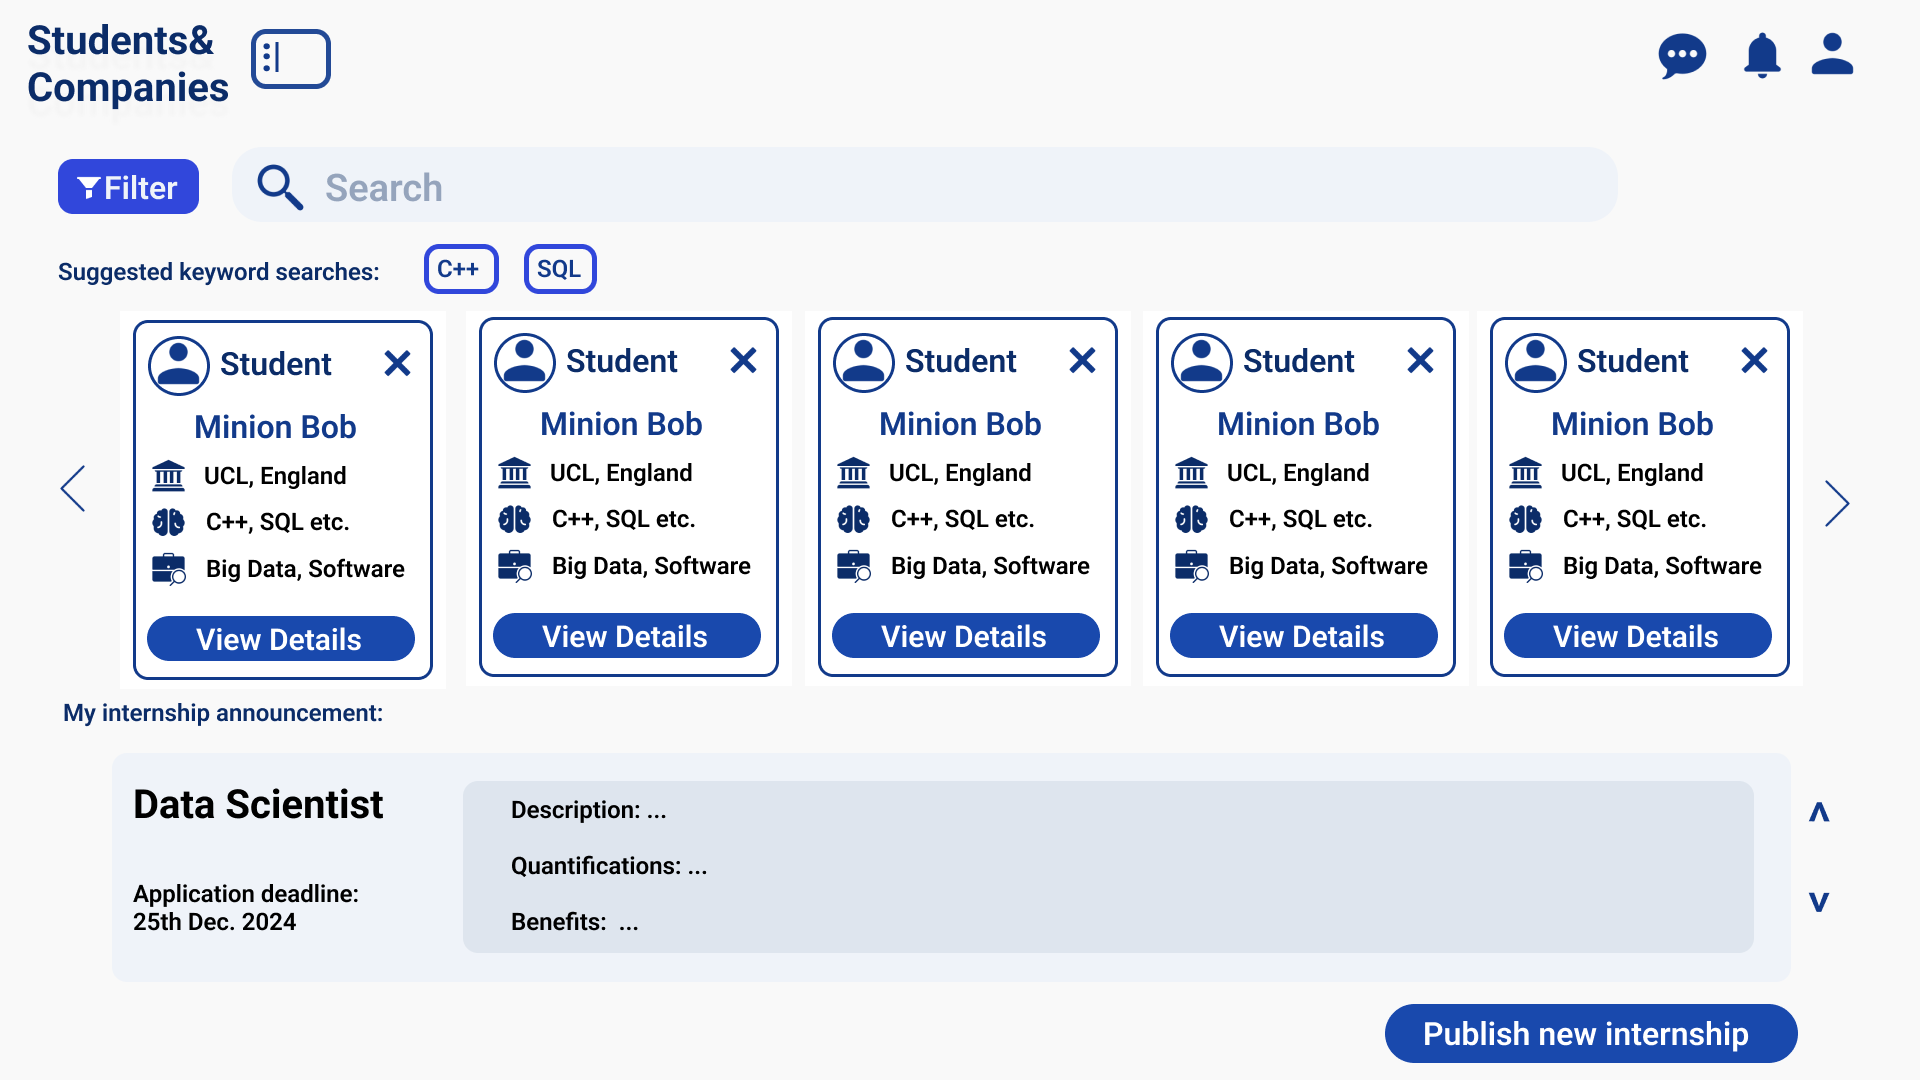
\includegraphics[width=0.8\textwidth]{Images/UI/Dashboard 1-company.png}
    \caption{Company's Dashboard 1}\label{fig:DashboardCompany1}
\end{figure}

\begin{figure}[H]
    \centering
    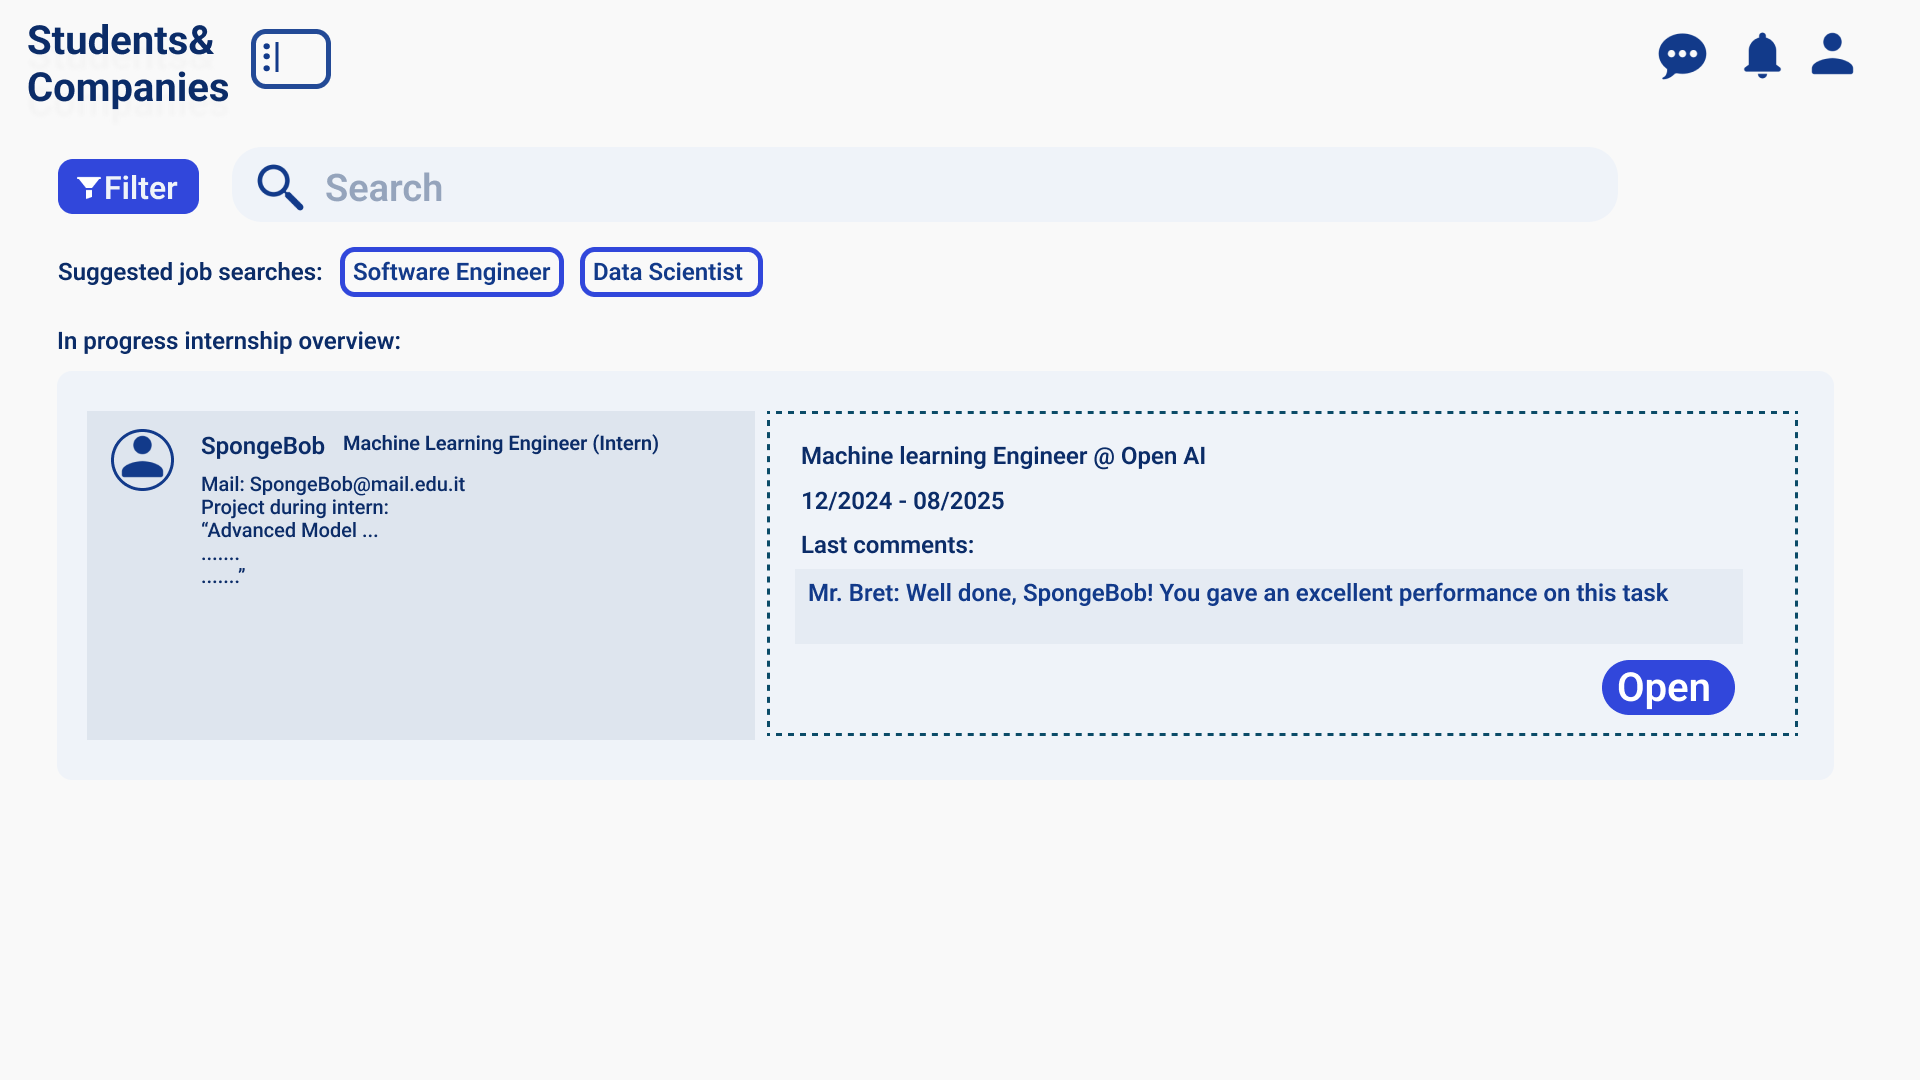
\includegraphics[width=0.8\textwidth]{Images/UI/Dashboard 2-company.png}
    \caption{Company's Dashboard 2}\label{fig:DashboardCompany2}
\end{figure}

\begin{figure}[H]
    \centering
    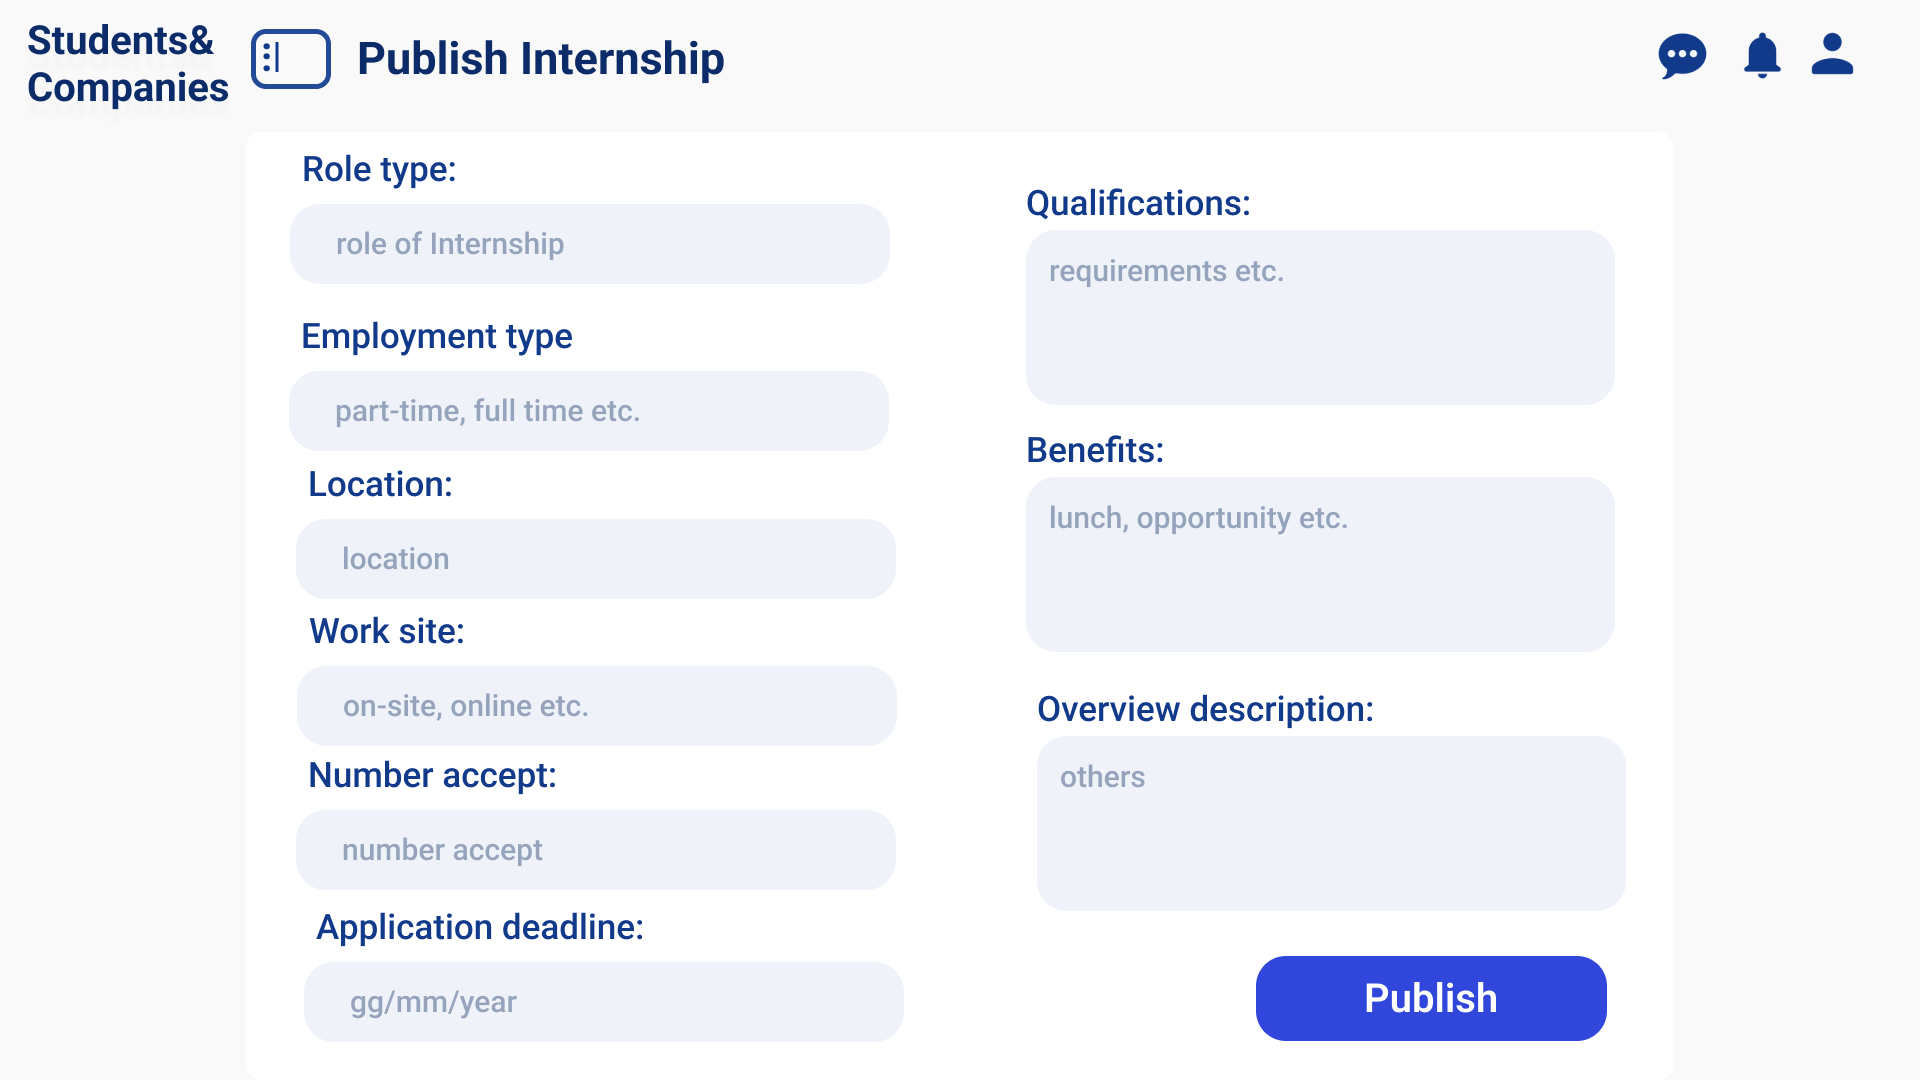
\includegraphics[width=0.8\textwidth]{Images/UI/Publish Internship -company.png}
    \caption{Publish Internship}\label{fig:Publish Internship}
\end{figure}

\begin{figure}[H]
    \centering
    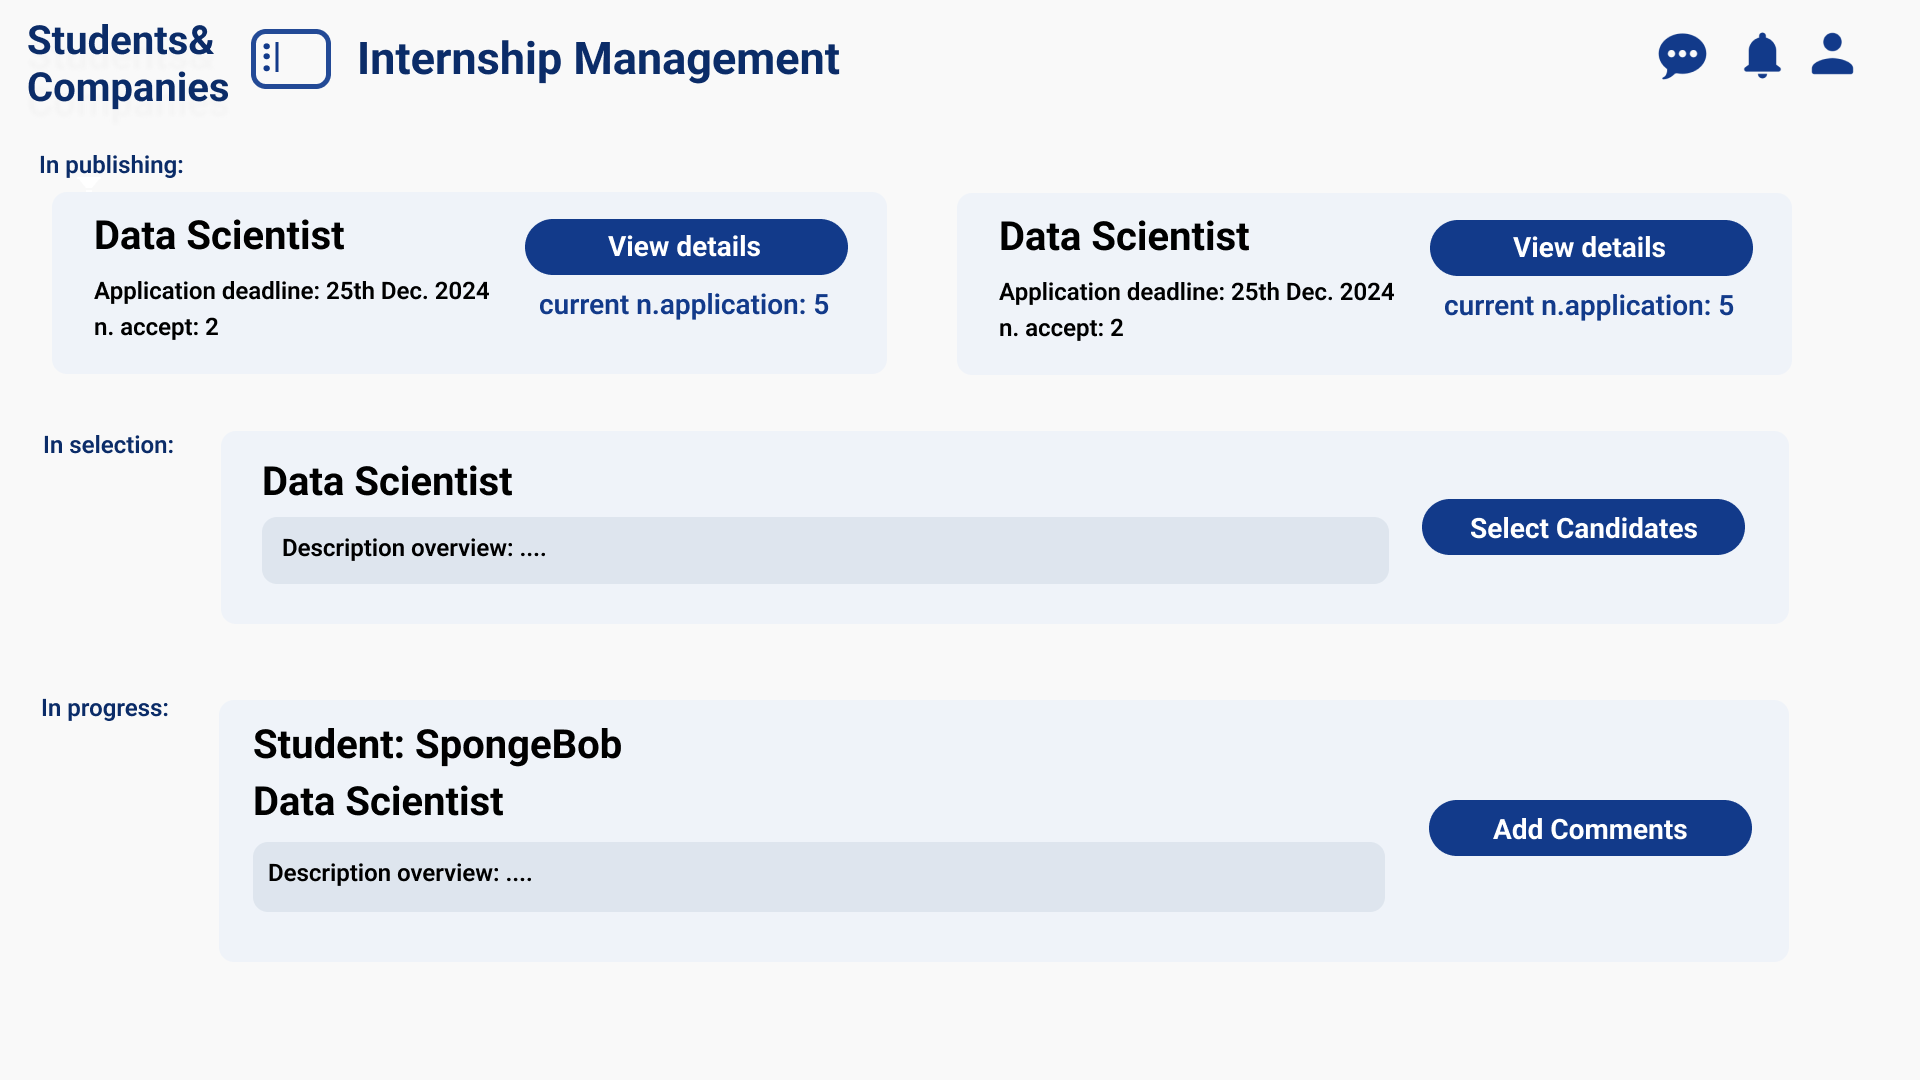
\includegraphics[width=0.8\textwidth]{Images/UI/Internship Management-company.png}
    \caption{Internship Management 1}\label{fig:Internship Management 1}
\end{figure}

\begin{figure}[H]
    \centering
    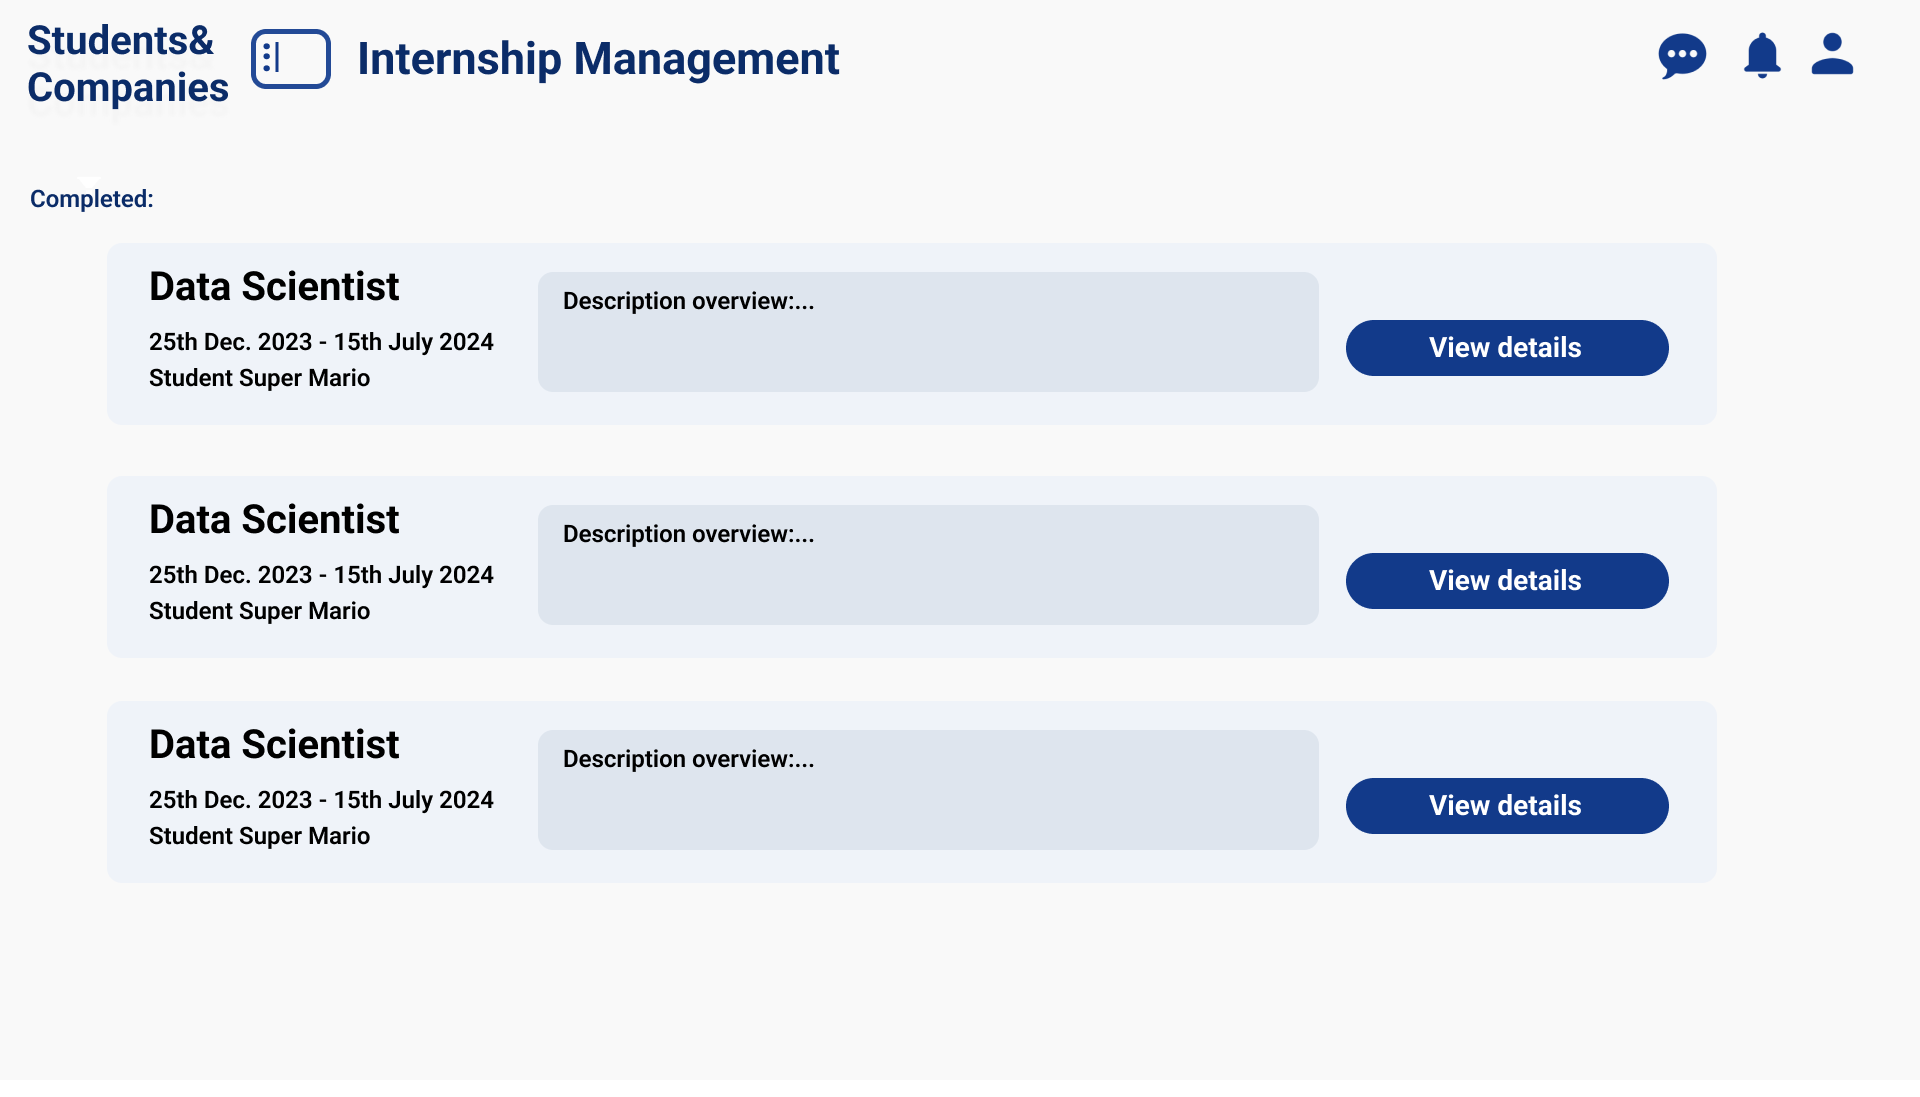
\includegraphics[width=0.8\textwidth]{Images/UI/Internship Management2-company.png}
    \caption{Internship Management 2}\label{fig:Internship Management 2}
\end{figure}

\begin{figure}[H]
    \centering
    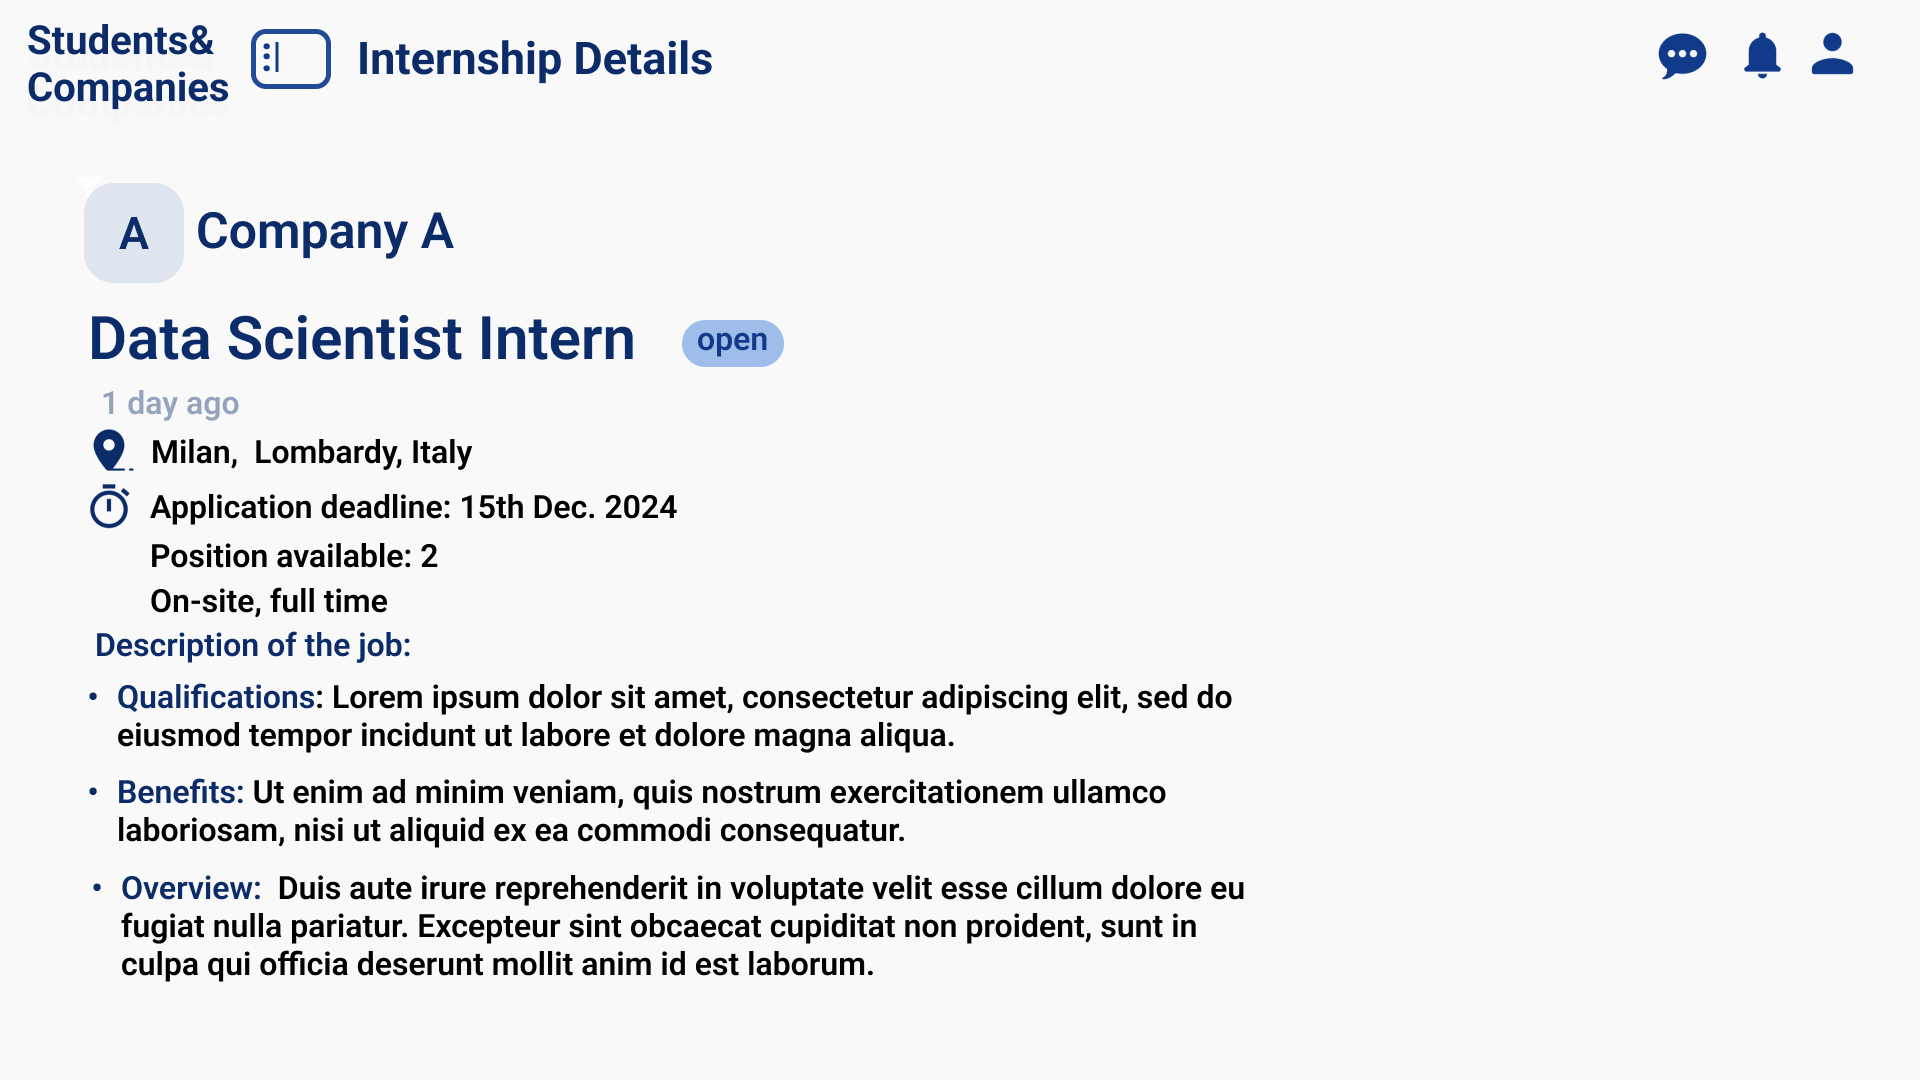
\includegraphics[width=0.8\textwidth]{Images/UI/Internship details-company view.png}
    \caption{Internship details in publishing phase}\label{fig:Internship details in publishing phase}
\end{figure}

\begin{figure}[H]
    \centering
    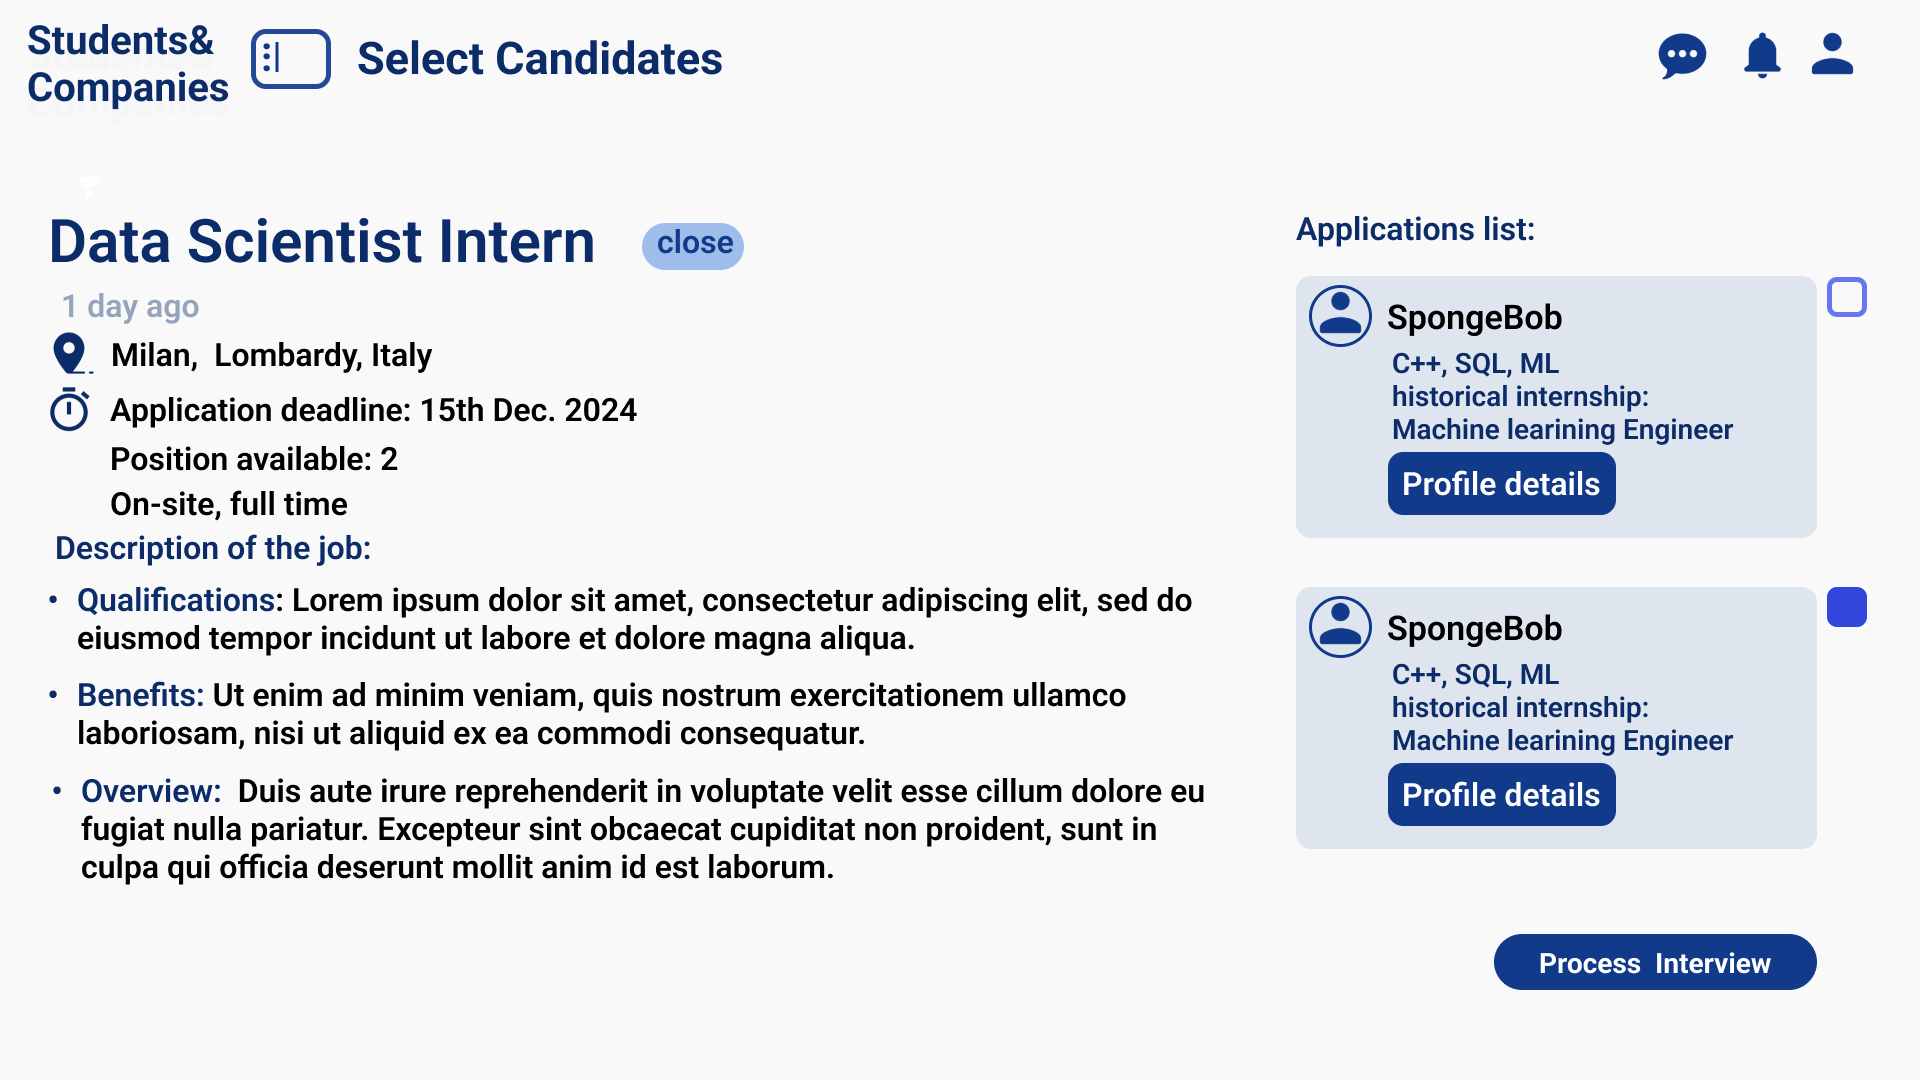
\includegraphics[width=0.8\textwidth]{Images/UI/Select candidates.png}
    \caption{Select candidates}\label{fig:Select candidates}
\end{figure}

\begin{figure}[H]
    \centering
    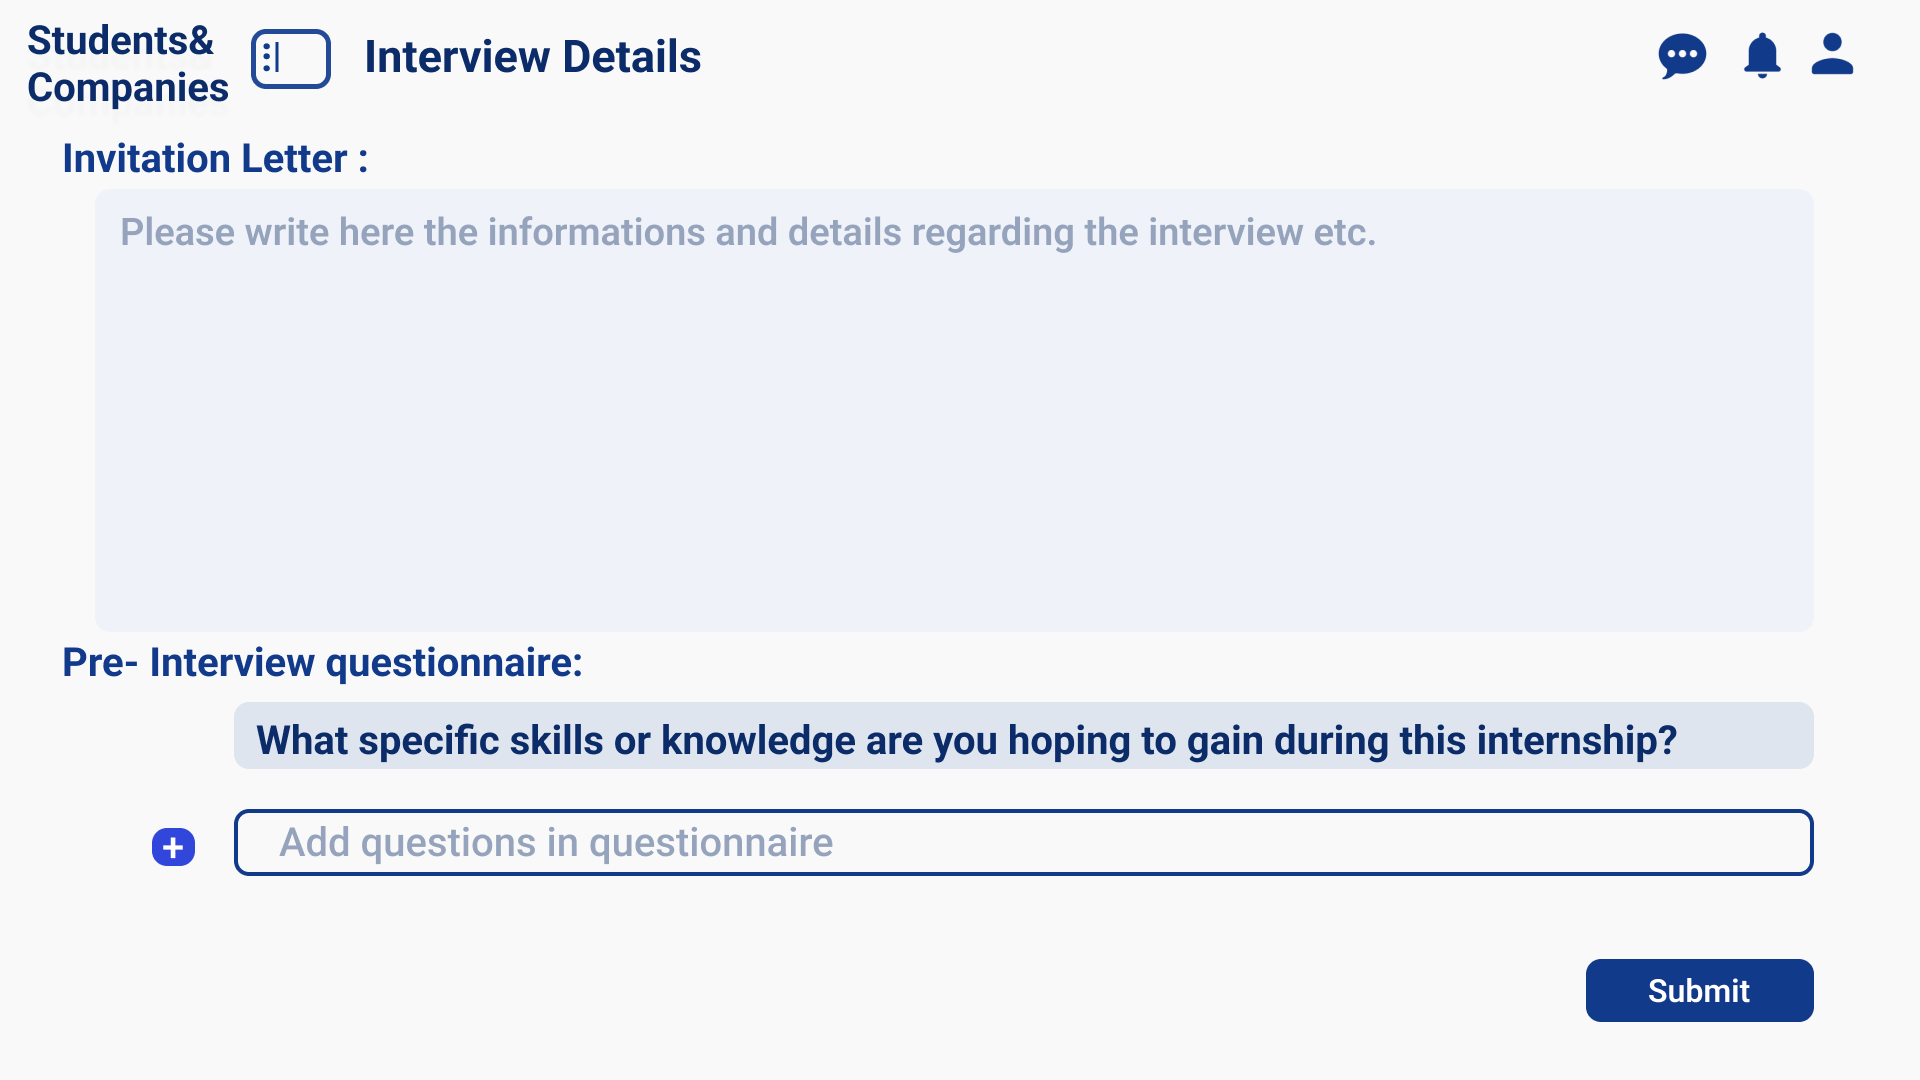
\includegraphics[width=0.8\textwidth]{Images/UI/Set Interview-Company.png}
    \caption{Set up interview}\label{fig:Set up interview}
\end{figure}

\begin{figure}
    \centering
    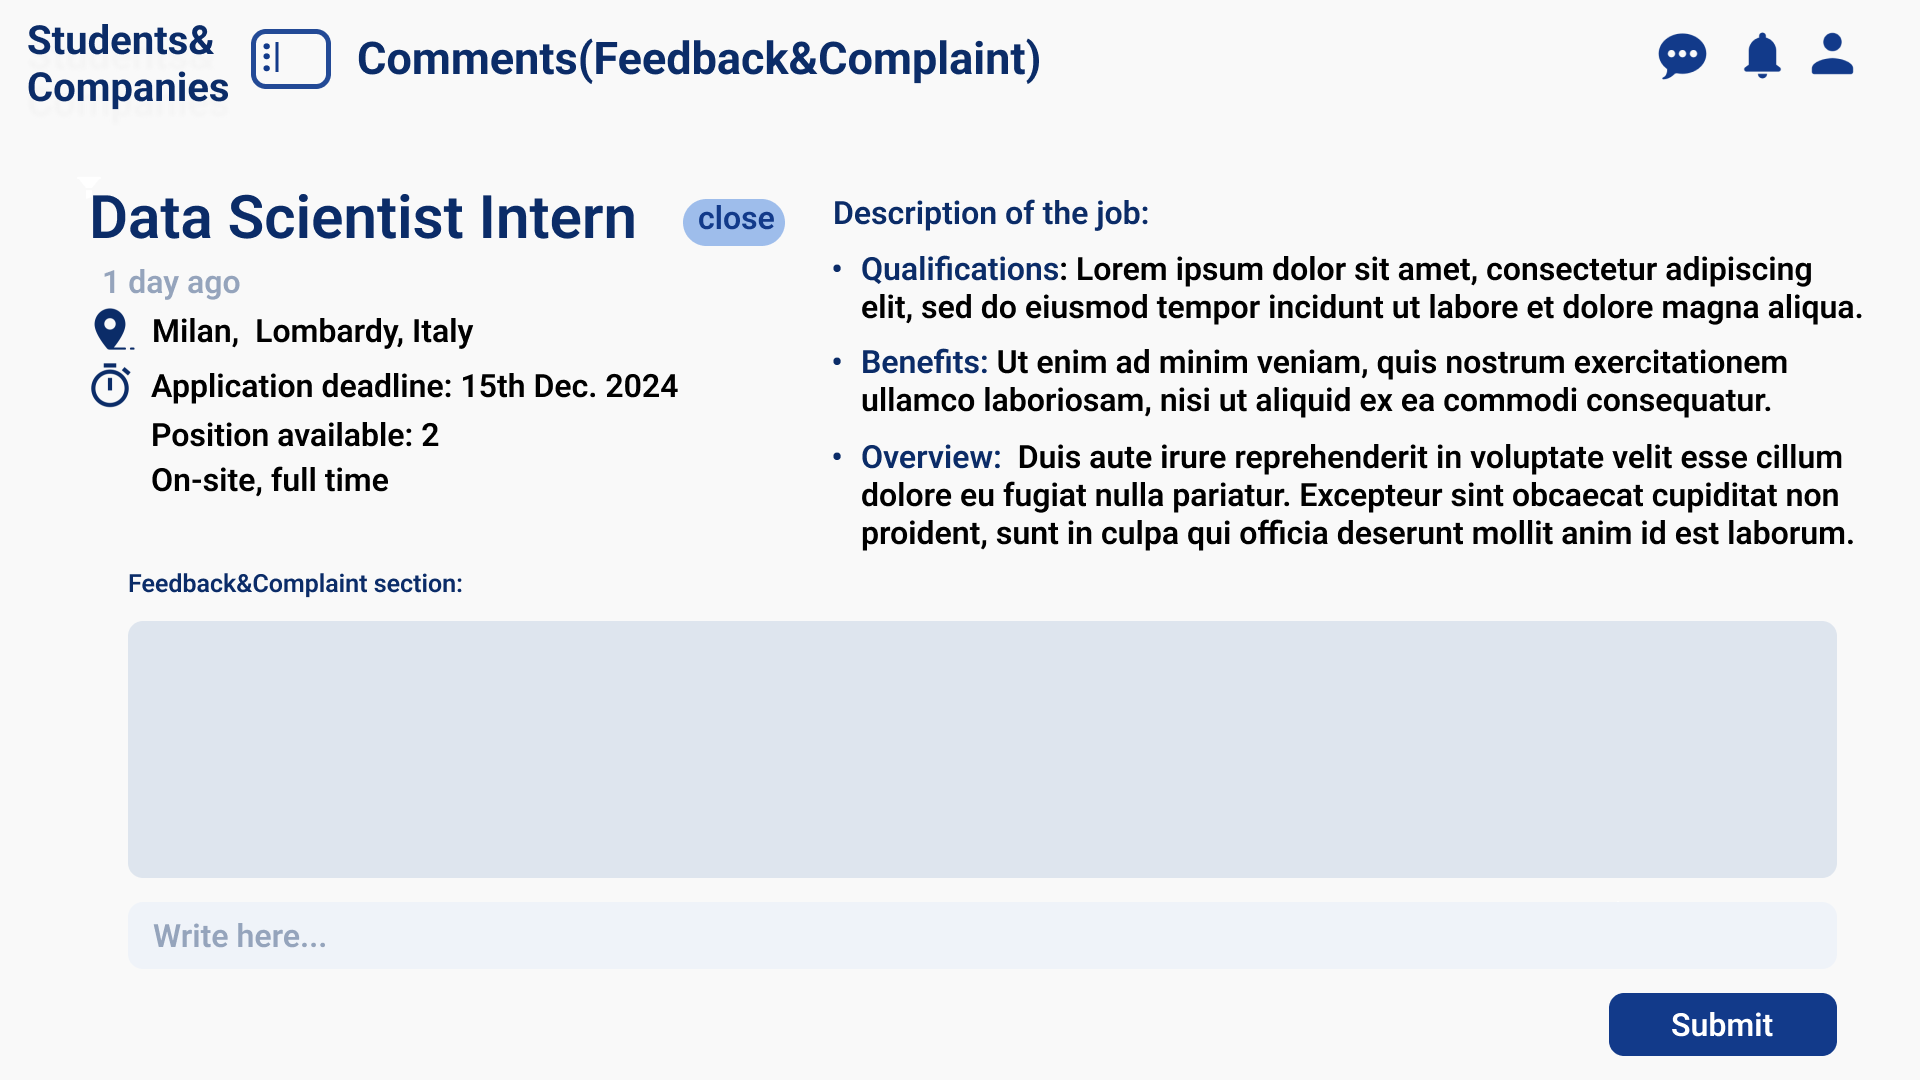
\includegraphics[width=0.8\textwidth]{Images/UI/FeedBack&Complaint- Student & Company.png}
    \caption{Feedback and Complaint}\label{fig:Feedback and Complaint}
\end{figure}


\begin{figure}
    \centering
    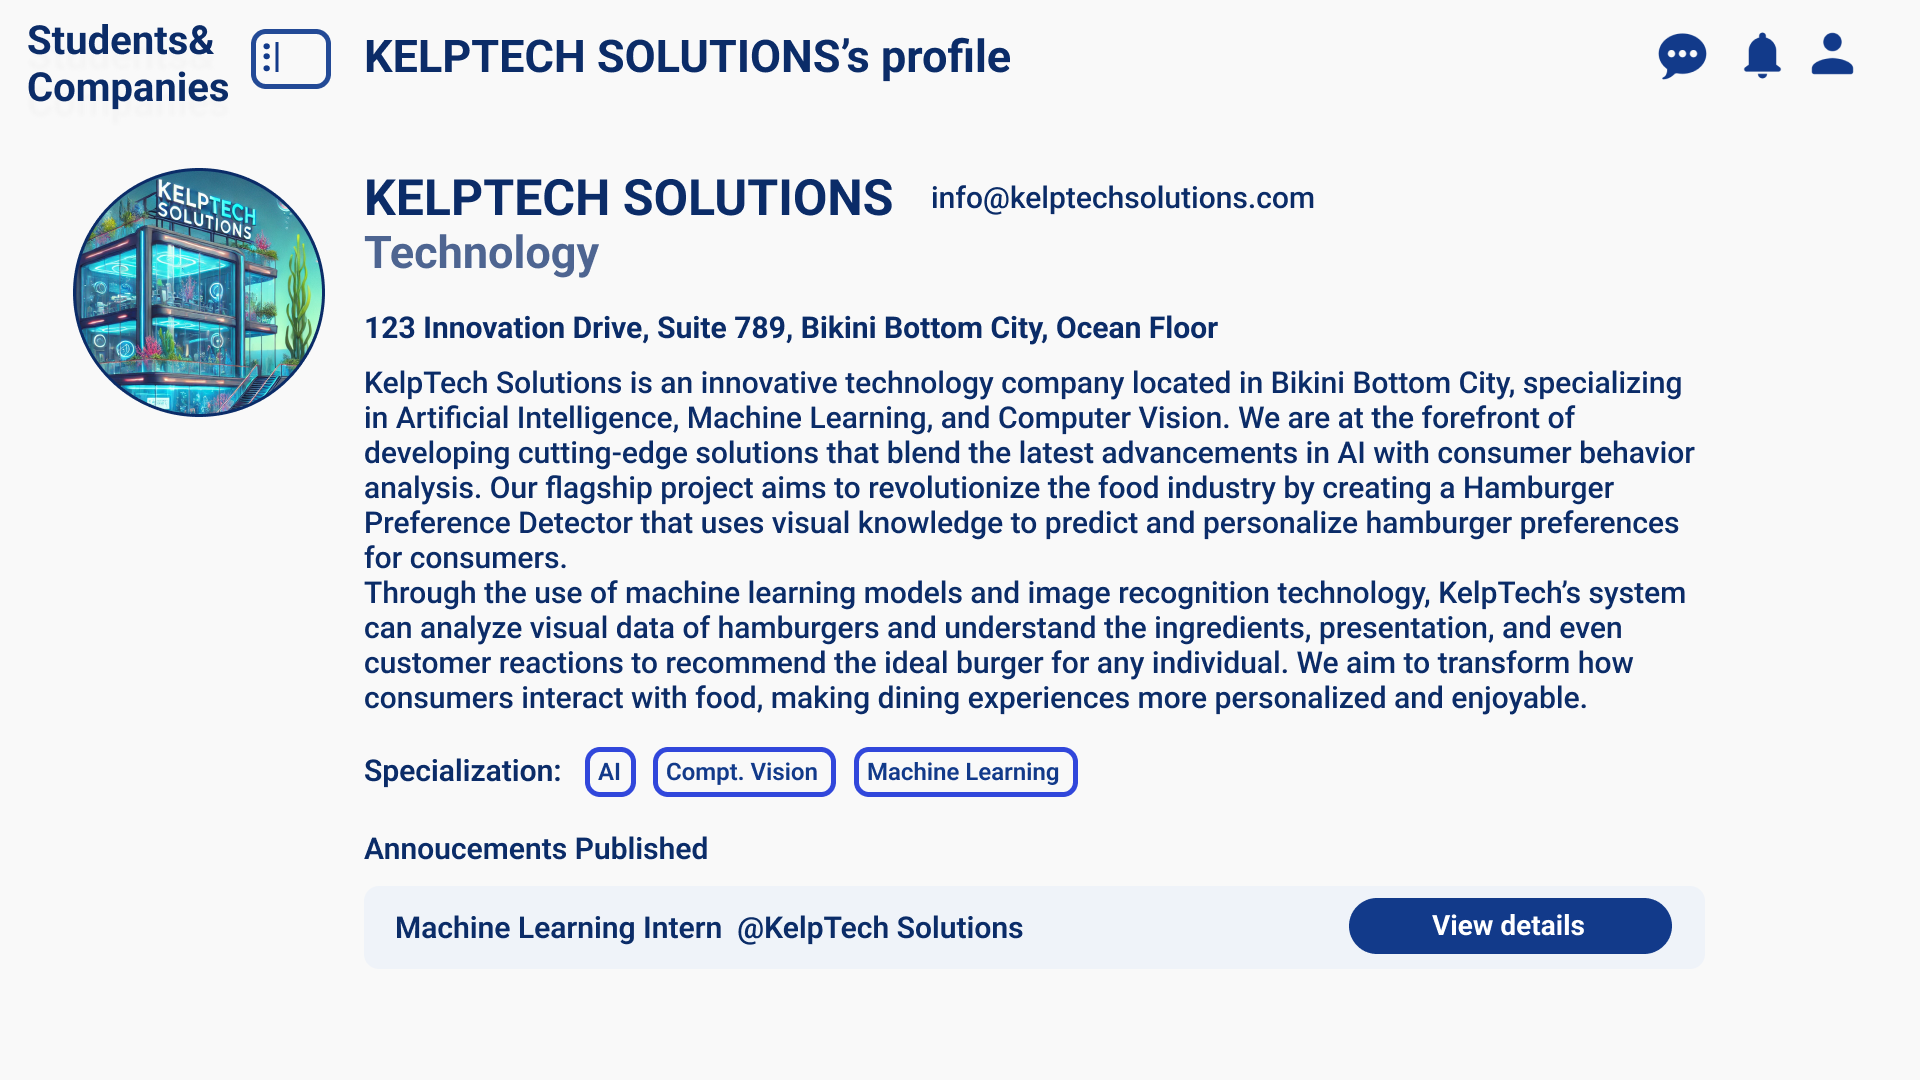
\includegraphics[width=0.8\textwidth]{Images/UI/Company profile.png}
    \caption{Company's profile from other's view}\label{fig:Company's profile from other's view}
\end{figure}


\subsection{University's view}

\begin{figure}
    \centering
    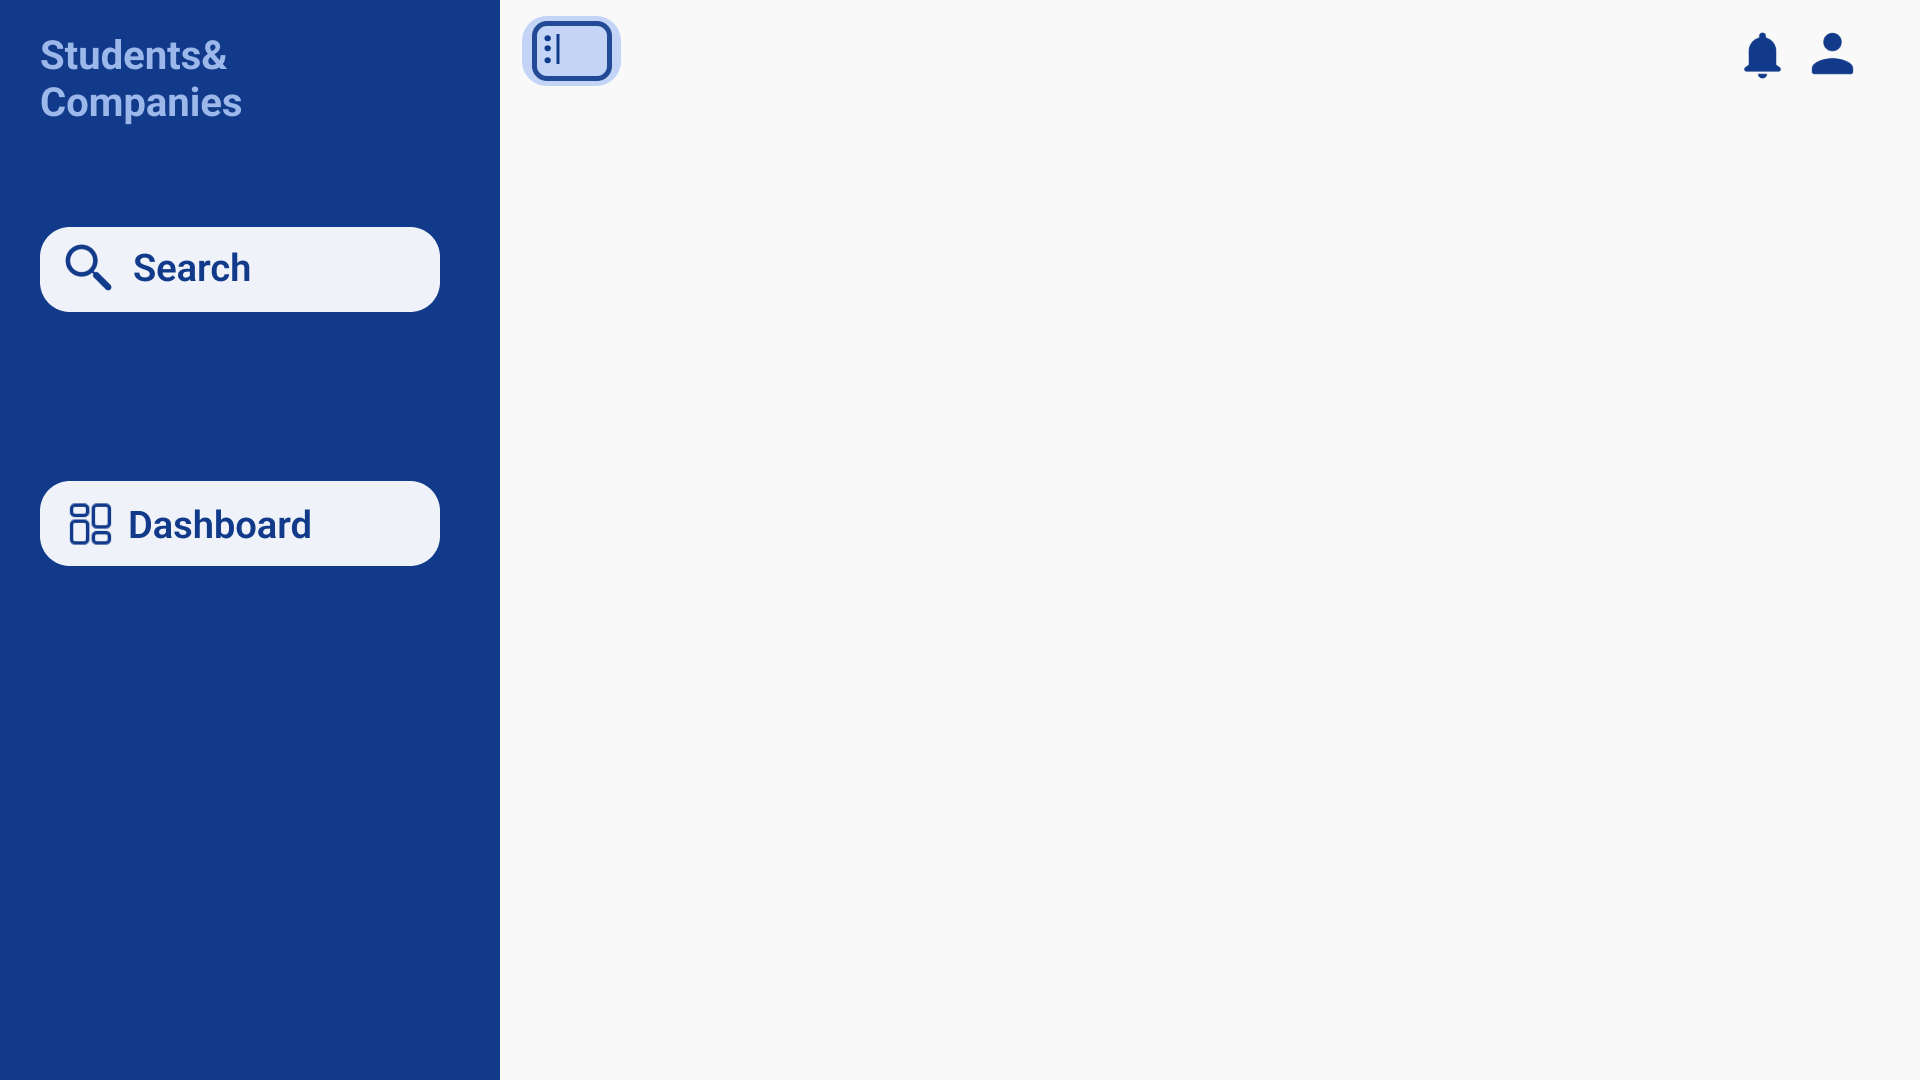
\includegraphics[width=0.8\textwidth]{Images/UI/Layout-University.png}
    \caption{University's Side Menu}\label{fig:University_view}
\end{figure}

\begin{figure}
    \centering
    \includegraphics[width=0.8\textwidth]{Images/UI/Dashboard 1-university.png}
    \caption{University's Dashboard 1}\label{fig:DashboardUniversity1}
\end{figure}

\begin{figure}
    \centering
    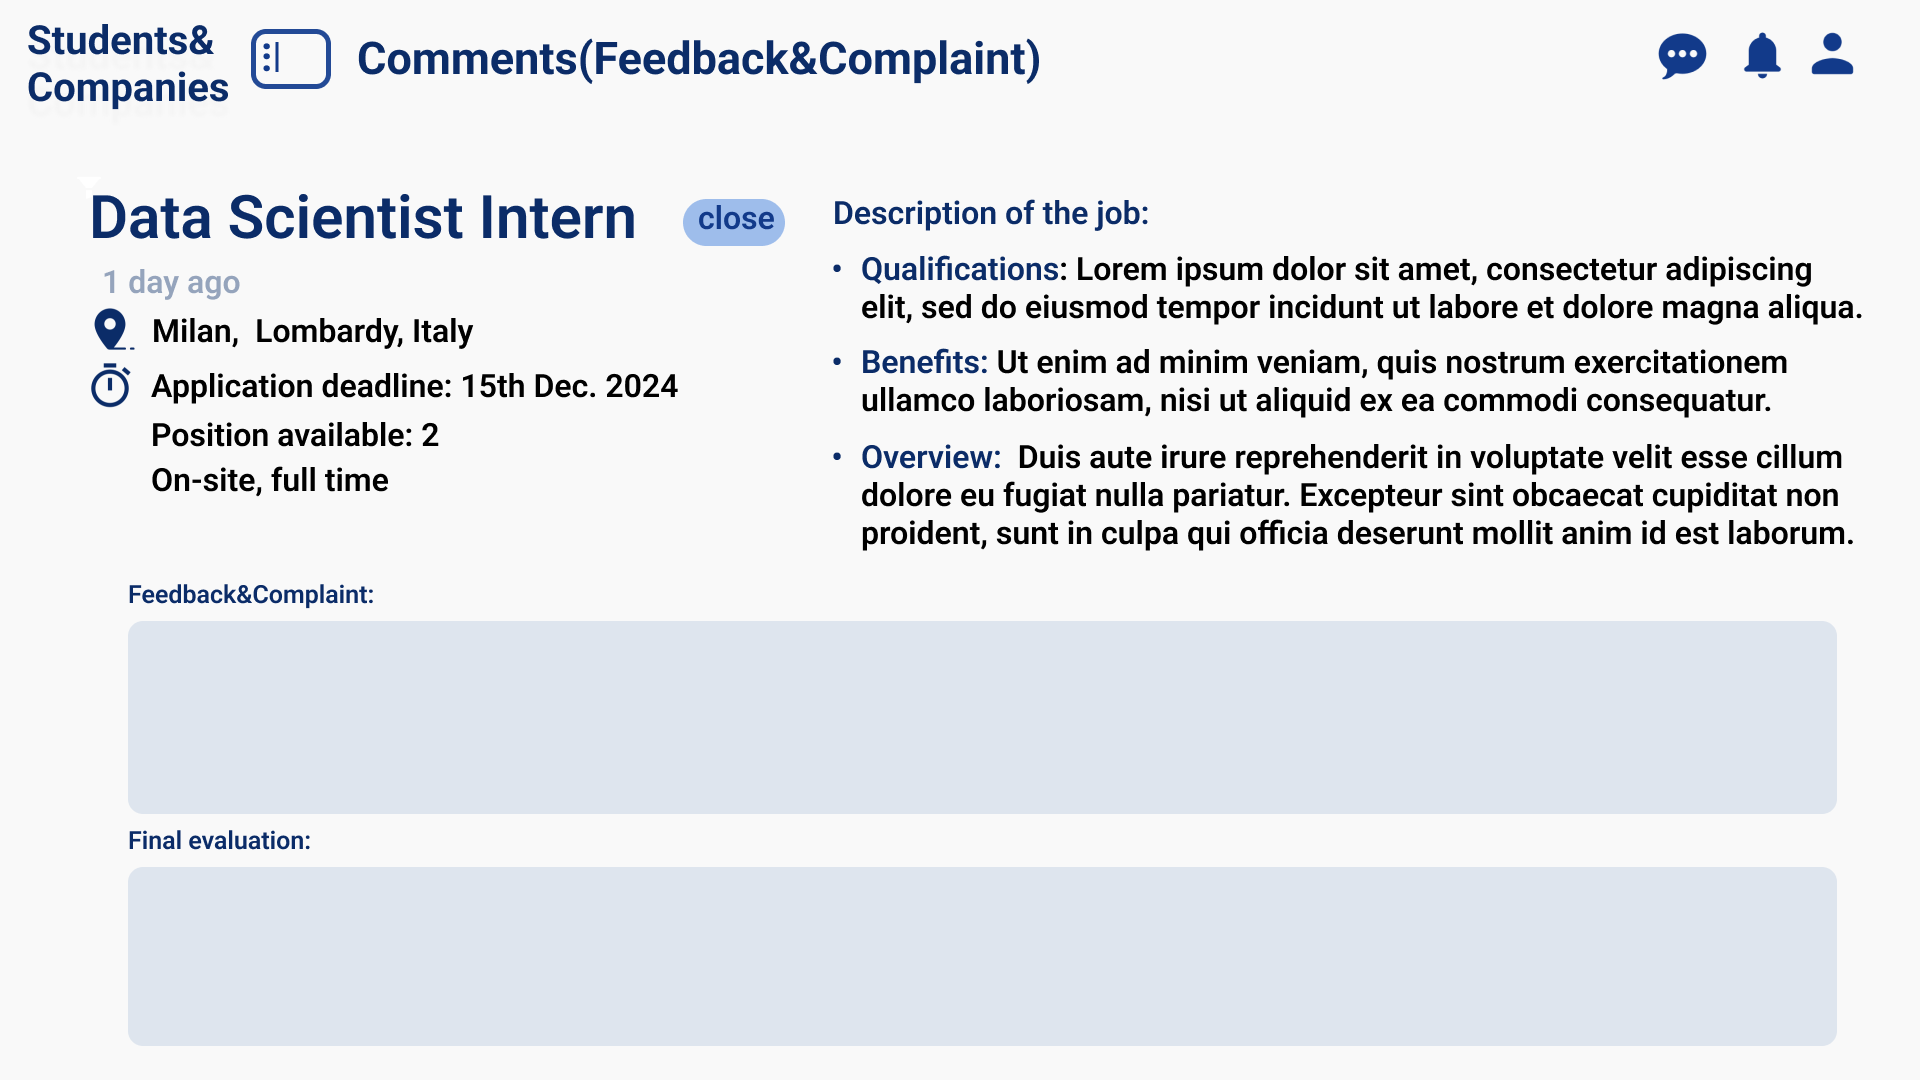
\includegraphics[width=0.8\textwidth]{Images/UI/FeedBack&Complaint- University view.png}
    \caption{Feedback and Complaint}\label{fig:Feedback and Complaint University}
\end{figure}